% Als Dokumentenklasse wird die 'report' Klasse von Koma-Script verwendet.
% Die Schriftgroesse kann hier eingestellt werden (10pt, 11pt, 12pt)
%\documentclass[a4paper,titlepage,12pt]{scrreprt}

\documentclass[a4paper,titlepage,11pt]{scrbook}
\KOMAoptions{captions=tableheading,parskip=full, headsepline=true, footsepline=false,
cleardoublepage=plain, headings=twolinechapter, numbers=noendperiod, appendixprefix=true,
chapterprefix=true}

%
% Hier werden benoetigte Pakete geladen. Manche sind nicht immer noetig und koennen 
% nach eigenen Geschmack entfernt werden. Zum experimentieren einfach die Zeile mit 
% einem '%' Zeichen auskommentieren.
%

\usepackage{ifpdf}% Gibt den Schalter \ifpdf, der angibt ob PDF oder DVI/PS ausgegeben wird.
\author{Dennis Reuling}

\usepackage[cmyk]{xcolor}%  Erweiterte Unterstuetzung von Farben. Die 'cmyk' Option behebt Farbprobleme wenn Transparenz verwenden wird.

\usepackage{filecontents}%  Erlaubt LaTeX-Code in andere Dateien zu schreiben

% zur Veränderung von Aufzählungszeichen (z.B. enumerate beginnend bei a),b),...)
\usepackage{paralist}

\usepackage{listings}

\usepackage{amsmath}

%customize the captions of floating environments
\usepackage[margin=10pt,font=small,labelfont=bf,textfont=sl]{caption}

\lstset{
    language=Java,
    keywordstyle=\bfseries\ttfamily\color{blue},
    identifierstyle=\ttfamily\color{black},
    commentstyle=\color[rgb]{0.457,0.723,0.0},
    stringstyle=\ttfamily\color[rgb]{0.627,0.126,0.941},
    showstringspaces=false,
    basicstyle=\footnotesize,
    numberstyle=\footnotesize,
    numbers=left,
    stepnumber=1,
    numbersep=4pt,
    tabsize=2,
    breaklines=true,
    keepspaces=true,
%   prebreak = \raisebox{0ex}[0ex][0ex]{\ensuremath{\hookleftarrow}},
    breakatwhitespace=false,
    aboveskip={1.5\baselineskip},
    columns=flexible,
    frame=single key,
    captionpos=b
    }

% Hyperref bzw. PDF Einstellungen (PDF links, Bookmarks, Info-Felder, etc.)
% Das 'hyperref' Paket wird verwenden. Einstellungen koennen mittels Paketoptionen,
% mittels \hypersetup{} oder mit der Konfigurationsdatei 'hyperref.cfg' veraendert werden.
% Manche Einstellungen muessen allerdings sehr frueh festgelegt werden und koennen spaeter
% nicht mehr veraendert werden. Der beste Platz diese festzulegen ist die Konfigurationsdatei die 
% vom Paket zur rechten Zeit eingelesen wird.
% Es wird die 'filecontents' Umgebung benutzt um die 'hyperref.cfg' mit den passenden Einstellungen
% zu erzeugen. Alternative kann dies auch manuell angelegt werden.
\begin{filecontents}{hyperref.cfg}
\hypersetup{
 pdfauthor={Dennis Reuling}
 pdfsubject={Integration of UML Profiles into the SiDiff and SiLift tools},
 pdfkeywords={UML, Profiles, Stereotypes, SiDiff, SiLift, SysML, AIS Case
 Study}, pdftitle={Integration of UML Profiles into the SiDiff and SiLift tools},
 backref=true,
 pagebackref=true,
 hyperfigures,
 hyperindex,
 bookmarksopen,
 bookmarksopenlevel=1,
 bookmarksnumbered,
 pageanchor,
 plainpages=false,
 % Hyperlink Farben:
 urlcolor=blue,
 pagecolor=black,
 menucolor=black,
 citecolor=green,
 anchorcolor=black,
 filecolor=black,
 linkcolor=black,
 colorlinks=true, % Links einfaerben oder umranden
}
\end{filecontents}
\usepackage{hyperref}% Hyperlinks 

%\usepackage{url}
% Normalerweise ist es nicht elegant, URLs nach einem Bindestrich zu trennen, aber 
% die lange URL zur PlaystationMoveMe-Referenz passt sonst nicht auf eine Seite
\def\UrlBreaks{\do\_\do-\do\/}

% ohne 'renewcommand{\backref}[1]{(S. {#1})}' stehen bei Verwendung von Bibtex im Literatur-
% verzeichnis lediglich die Seitenzahlen (ohne Zusatz 'S.') der Seiten, die die entsprechenden 
% Referenzierungen enthalten. 
\usepackage{backref}
\renewcommand{\backref}[1]{(S. {#1})}

\renewcommand*{\lstlistlistingname}{List of Listings}

\usepackage{pdfpages}% Andere PDF Dokumente einbinden (z.B. als Anhang)

\usepackage{graphicx}% zum einbinden von Bildern
% Definition von verwendeten Graphikformaten
\ifpdf
  \DeclareGraphicsExtensions{.pdf,.png,.jpg,.jpeg}
\else
  \DeclareGraphicsExtensions{.eps}
\fi
\graphicspath{{images/}{anhang/}}	% Pfade fr Grafiken angeben

\usepackage[english]{babel}%  Englische Sprache mit neuer Rechtschreibung

%\usepackage[ngerman]{varioref}% Definiert 

\usepackage[T1]{fontenc}      % T1 Schriften verwenden
\usepackage[utf8]{inputenc} % Erlaubt deutsche Umlaute in .tex Dateien. Je nach System kann statt 'latin1' auch 'utf8' o.a. verwendet werden
\usepackage{lmodern}          % Schriftart mit deutschen Umlauten

\usepackage{float} 

\usepackage{longtable} % Erlaubt ueberlange Tabellen ueber mehrere Seiten
\usepackage{flafter}   % Fliessumgebungen ('figure' and 'table') erst nach deren Deklaration verwenden.

\usepackage[printonlyused]{acronym} % Abkuerzungsverzeichnis


%%%%
% Stileinstellungen
\usepackage{setspace} % 
%\singlespacing%    Einfacher Zeilenabstand
\onehalfspacing%    1 1/2 Zeilenabstand (entspricht angeblich den doppelten Zeilenabstand in Word)
%\doublespacing%    Doppelter Zeilenabstand

\frenchspacing%     Kein doppeltes Leerzeichen nach '.' etc.
%%%%

% Mit folgenden Werten kann man die Silbentrennung einstellen (0..10000).
%\hyphenpenalty=10000 
%\exhyphenpenalty=10000
%\hyphenpenalty=10 \exhyphenpenalty=10

\setcounter{secnumdepth}{3}	% Hier stellt man ein bis zu welcher Ordnung berschriften nummeriert werden (Beginnt bei 0 (Kapitel) und geht bis 5 (Subparagraph)
\setcounter{tocdepth}{3}	% Hier stellt man ein bis zu welcher Ordnung berschriften ins Inhaltsverzeichnis bernommen werden (ebenfalls 0 - 5)
%

% Anzahl und max. Seitenanteil von Abbildungen und Tabellen einstellen
\setcounter{topnumber}{5}
\setcounter{bottomnumber}{5}
\renewcommand{\bottomfraction}{.9}
\renewcommand{\textfloatsep}{3ex}
\renewcommand{\floatsep}{3ex}

% Nicht empfohlene Einstellungen:
%\sloppy    % Schlampige Absatzformatierung (wie M$ Word)
%\usepackage{wordlike}    % Simuliert M$ Word 


%% Header-Layout
\pagestyle{headings}

%\usepackage{fancyhdr}
%\pagestyle{fancy}
%\addtolength{\headwidth}{\marginparsep}
%\headheight=35pt
%\fancyhf{}
%\renewcommand{\sectionmark}[1]{\markright{\thesection\ #1}}
%\lhead{\includegraphics[height=1cm]{ivr_logo_doku}\\
%Interactive Volume Rendering in Virtual Reality}
%\rhead{\rightmark}
%\renewcommand{\headrulewidth}{0.4pt}

% footer
%\rfoot{\thepage}

%redefine plain pagestyle - used for chapter pages.
%\fancypagestyle{plain}{
%  \fancyhf{}
%  \rfoot{\thepage}
%  \renewcommand{\headrulewidth}{0pt}
%}

% Erstelle Index
\makeindex

%------ the real document begins here ------
\begin{document}

%------ layout for title page ------

\pagenumbering{roman} % Roemische Kleinbuchstaben als Seitennummern (i,ii,iii,iv,v,vi,...). 'Roman' gibt Grossbuchstaben.

%------ preface, table of contents, summary ------
\begin{titlepage}
\ifpdf\pdfbookmark{Titlepage}{title}\fi	% Zum PDF Inhaltsverzeichnis hinzufügen
\begin{center}
  \includegraphics[scale=0.20]{logoSiegen} \\
  \vspace{3cm}
  \Large{\textbf{Master's Thesis}}
  \\
  \vspace{1cm}
  \huge{\textbf{ Integration of UML Profiles into the SiDiff and SiLift tools}}
  \\
  \medskip
  \Large{\textbf{Based on a SysML case study}}
  \\
  \vspace{2cm}
  \Large{Dennis Reuling} \\
  \vspace{4cm}
\textsf{
    \begin{large}
    \begin{tabular}{ll}
      Faculty: & Faculty of Science and Technology \\
      Department: & Electrical Engineering and Computer Science \\
      Institute: & Software Engineering Group\\
      Reviewers: & Prof. Dr. Udo Kelter, Dipl. Inf. Timo Kehrer \\
      Date: & \today
    \end{tabular}
  \end{large}
  }
\end{center}
\end{titlepage}

\chapter*{Abstract}\label{abstract}
\ac{MDSD} has become more 
and more present since the last years because of the paradigm shift
from coding to modeling. 
One of the most popular and commonly used modeling languages is the \ac{UML}. It
provides the possibility of extending the modeling language itself by
making use of the implemented \textit{profiling} mechanism. New elements with its own semantics can be added to
existing elements of the \ac{UML} thus enabling integration of new domains or
features easily.
A popular example for exploiting this mechanism is the \ac{SysML}, which extends the \ac{UML}
in the domain of systems engineering applications.

In the area of text-based tools the parallel work
paradigm has been used for the last decades. In the area of
model-based tools there have only be solutions which do not facilitate the freedom
or the functionality on par with the latter, which leaves many
features known to be desired. Three of these are the matching of corresponding
elements, the detection and presentation of differences and the creation
followed by the application of patches between two models.
The \textit{SiDiff} tool facilitates the first, whereas the
\textit{SiLift} tool provides the remaining two features.

This Master's Thesis introduces the integration of \ac{UML} profiles in both
tools:\\
Supporting a broad range of modeling languages and domains is crucial to
modeling tools in practicality. Therefore the integration of \ac{UML} profiles
is a significant enhancement in this area and is done in both tools for
supporting the whole processing pipeline: Beginning at the creation
of differences and concluding at the application of a patch.
A real world industrial automation case study using \ac{SysML} as modeling
language is presented and used as an exemplary input model to demonstrate the
final result of this integration process.

\chapter*{Statutory Declaration}
I declare on oath that I completed this work on my own and that information which has been directly
or indirectly taken from other sources has been noted as such. Neither this, nor a similar work, has
been published or presented to an examination committee.\\

Siegen, \today  \hspace*{5cm} \hrulefill

\chapter*{Acknowledgement}\label{acknowledgement}
\begin{quote}
%Leider läßt sich eine wahrhafte \\
%Dankbarkeit mit Worten nicht ausdrücken.\\
Wem die Dankbarkeit geniert,\\
der ist übel dran,\\
denke, der dich erst geführt,\\
wer für dich getan!\\
\textit{Johann Wolfgang von Goethe}
\end{quote}
\bigskip
%Ein Versuch ist es dennoch wert:\\
Ich möchte mich an dieser Stelle von ganzem Herzen bei meinen beiden Betreuern
Herr Prof. Dr. Udo Kelter und Herr Dipl. Inf. Timo Kehrer bedanken. Ohne sie und
ihre sowohl fachliche als auch menschliche Betreuung wäre diese Arbeit nicht
möglich gewesen. Auch den übrigen Mitarbeitern des Instituts der praktischen
Informatik bin ich zu tiefem Dank verpflichtet, welche mir stets zur
Seite standen.

Nicht vergessen möchte ich an dieser Stelle auch meine Kommilitonen, die mich
während dieses Lebensabschnittes begleitet und unterstützt haben. Während allen
Phasen des Studiums habe ich neue Freunde gefunden, welche auch außerhalb
fachlicher Fragen immer ein offenes Ohr hatten. Besonders erwähnt werden sollen
auch die Mitglieder des Fachschaftsrates, mit denen ich viel gemeinsame Zeit
verbracht habe, sowohl in der Rolle als Mitglied als auch in der Rolle als Freund.

Abschließend möchte ich den wichtigsten Menschen danken, meiner Familie
und meinen Freunden. Ihr wart stets an meiner Seite und habt mir erst dadurch
dieses Studium ermöglicht.

\begin{quote}
Vielen Dank!
\end{quote}
 


\ifpdf\pdfbookmark{\contentsname}{tableofcontents}\fi%   PDF Bookmark Eintrag fuer das Inhaltsverzeichnis.
{\singlespacing
\tableofcontents
}
\listoffigures   % Abbildungsverzeichnis
\lstlistoflistings
\chapter*{List of Abbreviations}
\renewcommand{\bflabel}[1]{\normalfont{\normalsize{#1}}\hfill}
\begin{acronym}
\setlength{\itemsep}{-\parsep}
\acro{API}{Application Programming Interface}
\acro{EMF}{Eclipse Modeling Framework}
\acro{HOT}{Higher-Order-Transformation}
\acro{ISO}{International Organization for Standardization}
\acro{LHS}{Left Hand Side}
\acro{MARTE}{Modeling and Analysis of Real Time and Embedded systems}
\acro{MDSD}{Model Driven Software Development}
\acro{NAC}{Negative Application Condition}
\acro{OMG}{Object Management Group}
\acro{PAC}{Positive Application Condition}
\acro{PPU}{Pick-and-Place Unit}
\acro{RHS}{Right Hand Side}
\acro{SCS}{Semantic Change Set}
\acro{SysML}{Systems Modeling Language}
\acro{SEG}{Software Engineering Group}
\acro{SERGe}{SiDiff Edit Rule Generator}
\acro{UML}{Unified Modeling Language}
\acro{UUID}{Universally Unique Identifier}

\end{acronym}
 % Abkuerzungsverzeichnis
\cleardoublepage
% Layout der Seiten
\pagenumbering{arabic} % Normale Seitennummern

%------ text of diploma thesis ------
\addcontentsline{toc}{chapter}{Introduction}
\pagestyle{plain}
\chapter*{Introduction}\label{introduction}
The paradigm shift from coding to modeling can easily be called one of the
biggest changes in progress in the area of software development. 
The main reason for this change has been the rising complexity of software,
whether it be in product families, different versions or the software itself.
Developers are trying to restrain this complexity by using modeling languages
and tools, which focus on the semantics of the given problem instead of
underlying programming languages.
Elevating the abstraction level eases the understanding of the problem and can
be one solution to cope with the rising complexity of software.

One important aspect to facilitate this paradigm shift is the definition of
modeling languages conforming to problems in practical domains of software. The
\ac{UML} has been introduced as such general-purpose modeling language and has
been accepted by the \ac{ISO} as industry standard for modeling
software-intensive systems since 2000. Although the modeling language already
supports many areas of software development like \textit{activities} or \textit{data modeling}, the \ac{UML} provides the generic facility for possible adaptions in
new areas or domains via its own \textit{profiling} mechanism: The \ac{UML} or
subsets of it can be extended by declaring own domain specific elements, adding
new properties to already existent modeling elements. The profiling mechanism is defined in an additive manner, therefore all profiled \ac{UML} elements are
still conforming to the \ac{UML} standard. Two popular examples of \ac{UML}
Profiles used by software developers in practice are \ac{SysML} and \ac{MARTE}.

Another important aspect for supporting \ac{MDSD} are the modeling tools
themselves, which should provide all needed and well-known features 
supported by text-based tools. To keep complex software manageable, there has to be the possibility to work in
sufficient large teams in parallel, without giving up the freedom of single
developers. Text-based tools are providing all necessary features for working
in teams since decades like the detection of correspondences and
differences between two revisions of software. The \textit{SiDiff} tool provides
such features for modeling languages: By implementing different
matching services, SiDiff can compute corresponding elements between two models
and is therefore the foundation of supporting parallel work in software
development. The \textit{SiLift} tool takes the support one step further in the
modeling tool pipeline: The detected differences are lifted upon a more
understandable level for the developer by presenting the changes via edit
operations. On this level of abstraction the changes are more comprehensive for
the developer,
which is crucial to parallel work paradigms. In the context of product families another feature is
well known from text-based tools, which has mostly been absent in the modeling
area: Patching of software. By making use of both SiDiff and SiLift another tool
has been developed, which facilitates this functionality in the modeling domain.
By supporting these three functionalities, \textit{Matching}, \textit{Lifting}
and \textit{Patching}, all basic features needed for parallel development are
available in \ac{MDSD}.

Supporting modeling languages, which conform to problems in
practical domains, in modeling tools, which facilitate well-known features in
parallel development areas, is a big step for the paradigm
shift to \ac{MDSD}. This Master's Thesis describes this integration process and
is structured as follows:

\textbf{Chapter \ref{environment_and_tools}} introduces the mentioned
environment consisting of the modeling language \ac{UML} including its profile
mechanism and the tools used for the integration.

\textbf{Chapter \ref{integration}} describes the concepts of the whole
integration process in a detailed manner, considering each pipeline step of the
modeling tools.

\textbf{Chapter \ref{realization}} illustrates the implementation of the
concepts described beforehand, whereas details and problems are
demonstrated.

\textbf{Chapter \ref{sysml}} analyzes a \ac{SysML} case study in a comprehensive
way, which will be used in the following chapter as input for testing the created solutions.

\textbf{Chapter \ref{solution}} sums up the integration success by
testing the solution using the case study described in the preceding chapter.

\textbf{Chapter \ref{conclusionfuturework}} considers the results from all
preceding chapters and presents a possible outlook and future work.



\pagestyle{headings}
\chapter{Definition of Environment and Tools}\label{environment_and_tools}
This chapter lays the foundation for all following chapters by introducing the
environment in which this Master's Thesis has been created. First the \ac{UML}
and its profiling mechanism is described, followed by a concrete
example in terms of \ac{SysML}.
Furthermore Henshin, a graph transformation tool used in this integration process, is
explained in detail. Finally the three target tools of integration are
presented:
\textit{SiDiff}, \textit{SiLift} and the \textit{Patch-Tool}.
\section{UML and UML Profiles}\label{environment_and_tools:umlprofiles}
In the early 1990's the rising paradigm of \ac{MDSD} demanded modeling languages
for all domains and use cases, in which software development came to practical
use. As in figure~\ref{mdsd_history} depicted, many modeling languages have been
developed in this era. One among them was the \ac{UML}, which has been developed
by \textit{Grady Booch}, \textit{Ivar Jacobson} and \textit{James Rumbaugh} at
Rational Software\cite{Wik13_1}. It differentiated itself from other modeling
languages in its generic ideas and its wide support for modeling domains. Its
special and important role has been lifted drastically in the year 1997, as the
\ac{OMG} adopted \ac{UML} as modeling language. They fine tuned
the language and presented their version to the \ac{ISO} afterwards. The
\ac{UML} has been accepted as standard and published as Version 1.3 in 2000,
which can easily be called one of the big milestones for \ac{UML} and even for
\ac{MDSD} in general. Before standarization the industry hesitated to choose one
of the many modeling languages for their own usage, because it takes time and
money to develop tools which can handle each modeling language with its own
semantics. The paradigm change from coding to modeling has been delayed until
the standarization of modeling languages like the \ac{UML}. The \ac{OMG}
developed new versions of \ac{UML} with new features ever since, the actual
stable version used in practical environments is \ac{UML} 2.4.1 and has been
released in August 2011\cite{OMGUMLSpecification}, which is also the version
used throughout this Master's Thesis. 
\begin{figure}[h!]
\begin{center}
\includegraphics[scale=0.4]{mdsd_history}\\
\end{center}
\caption{Modeling languages history~\cite{Wik13_1}}
\label{mdsd_history}
\end{figure}

The \ac{UML} has been designed with many generic principles in
mind\cite{OMGUMLSpecification} such as:
\begin{itemize}
  \item Modularity
  \item Partitioning
  \item Extensibility  
\end{itemize}
Making use of these principles the \ac{UML} can be used to visualize practical
problems in many domains, using elements in combination like \textit{activies},
\textit{components} or \textit{use-cases}. An example of an \ac{UML} class
diagram, which is a very popular type of diagram in general, can be seen in
figure~\ref{uml_classdiagram}. This Master's Thesis emphasizes only on the
important parts of \ac{UML} for the integration, a more detailed and
comprehensive description of all possibilities the modeling language has to offer can be found in
\cite{UMLNutshell}.
\begin{figure}%[h!]
\begin{center}
\includegraphics[scale=0.5]{uml_classdiagram}\\
\end{center}
\caption{\ac{UML} class diagram example~\cite{Wik13_2}}
\label{uml_classdiagram}
\end{figure}

Although the \ac{UML} supports a wide range of modeling domains, the principle
of \textit{extensibility} has been integrated deeply with its own mechanism: The
\ac{UML} profiling mechanism. The idea behind this mechanism is the possibility
for developers to define own modeling elements in \ac{UML} notation and
therefore add new semantics to an already known and widely supported modeling
language such as the \ac{UML}. Instead of defining a own modeling language for a
new given domain from scratch, a defined profile can alter a (sub)set of \ac{UML}
to provide a semantically more unterstandable way of modeling or additional
features, which have been missing in this particular area. An example of such an
profile definition is presented in figure~\ref{uml_profileexample}: Servers are
defined as profile for better understanding in this modeling domain. They extend
the \ac{UML} with its own semantics, such as the relationship between a
\textit{device} and a \textit{server}. 
\begin{figure}%[h!]
\begin{center}
\includegraphics[scale=3.5]{uml_profiled}\\
\end{center}
\caption{Profile Application Example~\cite{UMLprofiled}}
\label{uml_profileexample}
\end{figure}

All \ac{UML} profiles are defined in an \textit{additive} manner. This basic
principle leads to conformity between unprofiled and profiled \ac{UML} models, therefore no new modeling tools are
needed if they already support all features of \ac{UML}. This is a tremendous
advantage over other modeling languages, which do not facilitate such
extensibility in this generic way or at all. Another example exposing this can
be imagened easily:
The technology of connected devices like tablets or new server backends like clouds are using a
new way of network connectivity. To cope with this new area of problems in a
\ac{MDSD} way there has to be a modeling language and modeling tools capable of
such modeling elements and their relationships. Using the \ac{UML} profiling
mechanism no new modeling tools are needed, all semantics of this new domain
are modelled within \ac{UML} profiles, such as relationships between cloud
servers and its clients.

These are just small examples of what possibilities are available via the
profiling mechanism. Other popular examples which are using this functionality extensively are \ac{MARTE} and \ac{SysML}, which will be explained in detail in the
following section.
\section{SysML}\label{environment_and_tools:sysml}
One example of making use of the \ac{UML} profiling mechanism is the \ac{SysML}
profile, which defines new semantics to existing elements in the \ac{UML} and
extents the modeling language with new elements and diagrams. The profile is
used in  and has been developed for the domain of systems engineering applications.
Like \ac{UML}, \ac{SysML} has been adopted by the \ac{OMG} and its specification
has first been published officially in September 2007\cite{Wik13_3}. The current
version in use is \ac{SysML} 1.3, which was issued by the \ac{OMG} in June 2012
\cite{OMGSysMLSpecification}.

\ac{SysML} tries to reduce the scope of modeling elements of \ac{UML} by using
only a subset of all elements available as depicted in figure
\ref{sysml_uml_relation}. The wide support of modeling domains and elements of
\ac{UML} can lead to confusion among developers, which \ac{SysML} tries to solve
by only using domain specific elements in the area of systems engineering.

\begin{figure}%[h!]
\begin{center}
\includegraphics[scale=0.4]{sysml_uml_relation}\\
\end{center}
\caption{Relationship between \ac{UML} and \ac{SysML}~\cite{OMGSysML}}
\label{sysml_uml_relation}
\end{figure}

Additionally parts of \ac{UML} have been changed in semantics and new diagrams
have been introduced. A \ac{SysML} diagram overview is presented in figure
\ref{sysml_overview}.

\begin{figure}[h!]
\begin{center}
\includegraphics[scale=0.5]{sysml_overview}\\
\end{center}
\caption{The SysML diagram taxonomy~\cite{OMGSysMLSpecification}}
\label{sysml_overview}
\end{figure}

 The new diagrams introduced in \ac{SysML} shall be explained:
 
\textbf{Requirement Diagram}\\
Systems engineering is mostly driven requirement-based, therefore this new type
of diagram meets this design principle. In this domain a requirement can be
modeled graphically and contains properties and/or conditions which must be
satisfied. Requirements can have relationships between modeling elements, which
can also be requirements themselves. Another feature is the reuseability across
product families and projects, which is realized through the namespace
containment in \ac{SysML}.

\textbf{Parametric Diagram}\\
As seen in figure~\ref{sysml_overview}, the parametric diagram has a direct
relationship to the internal block diagram, which contains the basic modeling
elements of \ac{SysML}. The idea is to offer the possibility to describe
constraints among properties between these basic elements such as
\textit{Blocks}.
Behavior and structure models can be integrated easily with engineering analysis like
performance or reliability, which often occur in systems engineering domains.

Additionally many modififications have been implemented to conform to the
systems engineering common language and principles in software design, making
them more understandable for developers from this particular domain. A basic
example for this is the \ac{UML} \textit{Class} element extension by
the \ac{SysML} \textit{Block} element. This seems appropiate because of the common usage of mechanical or electrical parts, which do not conform to the semantic of \textit{Class}.
A more detailed overview and description of all elements, which are
introduced by \ac{SysML} and how they are used can be found in
\cite{OMGSysMLSpecification} and~\cite{SysMLEngineering}.
\section{Henshin}\label{environment_and_tools:henshin}
Contrary to text-based tools, modeling tools are based on graph
representations as input. A model can be defined as graph, consisting
of nodes representing the modeled element instances and edges representing
relationships between them. Henshin is built upon this foundation of model representation,
whereas the name Henshin originates from Japanese and translates to
\textit{transformation}.
It has been developed as a joint project by developers at the
Philipps-University in Marburg, the Hasso Plattner Institute in Potsdam, 
the Technical University of Berlin, and others~\cite{Henshin}. The first version
of Henshin, 0.8.0, has been released in September 2011, and Henshin has been in
development ever since. The current stable version is 0.9.8, which this Master's
Thesis uses throughout the whole integration process. 

Based on the theory of graph transformation\footnote{Often also
called graph rewriting}, Henshin provides the functionality of transformating a
given model based on defined Henshin rules. The tool itself is implemented for
the \ac{EMF} and can be used within this context. Like compilers in text-based
tools, graph-transformation tools are trying to find a match on the \ac{LHS} and transformate this match
based on a given rule into a result on the \ac{RHS}. In figure~\ref{graphrewriting_example} the \ac{LHS},
denoted as $L$ is transformed into the \ac{RHS} denoted as $R$. A
multiplication with $2$ is transformed into an addition of the digit with
itself. The corresponding match on the \ac{LHS} and result on the \ac{RHS} are
denoted in dashed lines. This rudimentary definition and example are sufficient
in this context, for a in-depth view on graph transformation and the theory
behind~\cite{rozenberg1997handbook} can be recommended.

\begin{figure}%[h!]
\begin{center}
\includegraphics[scale=0.5]{GraphRewriteExample}\\
\end{center}
\caption{Graph transformation example~\cite{Wik13_4}}
\label{graphrewriting_example}
\end{figure}

For using Henshin the definition of Henshin rules is essential: Henshin rules
are used as input language for the transformation process, additionally to the
input model itself. Using the graphical Henshin diagram syntax, a defined rule
looks similar to the example rule in figure~\ref{Henshinrule_example_1}. There are
five types of nodes in a Henshin rule, whose semantics correspond to the five
type of edges:
\begin{itemize}
  \item \textbf{Create} \\
  	    A create node exists only in the \ac{RHS} of the input model and is
  	    therefore created in the result model.
  \item \textbf{Delete} \\
  	    A delete node exists only in the \ac{LHS} of the input model and is
  	    therefore deleted from the input model.
  \item \textbf{Preserve} \\
        A preserve node exists in both sides of the input model, \ac{LHS} and
        \ac{RHS} that is. These nodes are used as a match in \ac{LHS} and are not altered in the result model.
  \item \textbf{Forbid} \\
        A forbid node, or \ac{NAC}, defines which
        elements are not allowed to be matched in the \ac{LHS} for executing the
        transformation. If one forbid node is found in the input model, the
        transformation can not be executed.
  \item \textbf{Require} \\
        A require node, or \ac{PAC}, defines which
        elements must be matched in the \ac{LHS} for
        executing the transformation. If one require node is not found in the
        input model, the transformation can not be executed.
\end{itemize}
\begin{figure}[h!]
\begin{center}
\includegraphics[scale=0.4]{rule-create-account}\\
\end{center}
\caption{Henshin rule example (1)~\cite{Henshin}}
\label{Henshinrule_example_1}
\end{figure}

Using these types of nodes and edges, describing relationships between
nodes, one can use Henshin for transformating a given input model.
The example shown in figure~\ref{Henshinrule_example_1} creates a bank account
for a client by transformating a given input model conforming to a meta model
describing a bank and its relationships to its accounts, managers and clients.
The forbid node on the left represents the constraint that no two accounts managed by the same bank may
have the same account id. The parameters which are given to the Henshin rule
should also be mentioned, they can be a primitive type like a \textit{String} or
a object parameter and are used for the execution. The transformation engine of
Henshin itself executes a Henshin rule as follows:
\begin{enumerate}
  \item Search for a match in input model, defined via preserve nodes and their
  relationship to other nodes.
  \item Check if no forbid node could be matched or a require node could not be
  matched.
  \item Create all create / delete all delete nodes and edges describing their
  relationship.
\end{enumerate}
A special feature of Henshin Rules are presented in figure
\ref{Henshinrule_example_2}: Nested rules. The delete node is marked with a
star operator and therefore will be executed as many times as possible. In this
particular example all accounts of a client will be deleted instead of only
one as if not defined as nested rule. Internally the Henshin interpreter will
try to match the preserve nodes and edges after each successfull execution and
if it succeeds, it will execute the transformation again. This feature is important
for later use and therefore is explicitly mentioned and explained.
\newpage
\begin{figure}[h!]
\begin{center}
\includegraphics[scale=0.5]{rule-delete-all-accounts}\\
\end{center}
\caption{Henshin rule example (2)~\cite{Henshin}}
\label{Henshinrule_example_2}
\end{figure}

Using Henshin as a tool, it offers different ways of executing Henshin
rules for transformation. They can be executed either via the Henshin
graphical interface, or via the Henshin interpreter \ac{API}, which can be
called using programming languages like Java. All described tools in this
Master's Thesis are based on the latter option. Because Henshin offers more
features than described in this section, publications of the developers of
Henshin like~\cite{henshinpublication} are recommended as additional lecture.
\section{SiDiff}\label{environment_and_tools:sidiff}
As mentioned in the introduction do modeling tools need to support features
known from text-based tools. One important aspect for parallel development
paradigms is the detection of correspondences and differences between two
different revisions of software. In the area of \ac{MDSD} 
software consists of models, therefore such features must be available in this
context. The SiDiff tool environment~\cite{SiDiffURL} offers such
functionalities: It can derive correspondences and differences between two
models meta model-independent. The basic concept and tool implementation was
released in 2004 by the \ac{SEG}~\cite{SEGURL}, whereas this version can be
defined as proof of concept. The version in today's use was initiated in 2009,
it has been revamped from scratch and implements a new software architecture
built upon \textit{OSGi} and the Eclipse plugin ecosystem. SiDiff is built upon
a service-based architecture internally, which eases the integration of new
services in any part of the computing pipeline including the matching itself.
\newpage
\begin{figure}[h!]
\begin{center}
\includegraphics[scale=0.5]{sidiffworkflow}\\
\end{center}
\caption{SiDiff workflow~\cite{SiDiffURL}}
\label{sidiffworkflow}
\end{figure}

SiDiff make use of the computing pipeline depicted in figure
\ref{sidiffworkflow}: Two models are used as input for comparison and are
annotated for later processing of the implemented matching services. One big
advantage of SiDiff is its vast configuration possibility, which emphasizes
its generic approach. In this step of pipeline the configuration defines which
model elements are annotated and how this is done. The SiDiff matching services
are then computing correspondences on the resulting annotated
models, whereas the current available matching services consist of:
\begin{itemize}
  \item  \textbf{ID-based Matcher} \\
  		This matcher makes use of given \ac{UUID}s, if available. Elements of Model
  		$1$ are corresponding to Elements of Model $2$ if and only if their
  		respective \ac{UUID} is equal.
  \item  \textbf{Signature-based Matcher} \\
  	 	This matcher is based upon signatures of elements, which can be computed by
  	 	taking attribute values or relationships into consideration. Which
  	 	properties are used for the creation of signatures is defined via a
  	 	configuration file.
  \item  \textbf{Similarity-based Matcher} \\
  		This matcher computes a similarity between elements, and if they reach a
  		given threshold they are declared as corresponding. This part of SiDiff
  		can be configurated in enormous detail, for example which element attributes
  		are weighted in comparison to others. This matcher and its
  		configuration is to comprehensive to discuss in detail, a more
  		detailed look is given in~\cite{KellerWN05}.
\end{itemize}
The matching result defines which elements of Model $1$ are  corresponding to
which elements of Model $2$ only, therefore a difference engine is executed
afterwards for detecting unmatched elements. The final result is a 
symmetric difference, which consists of both the correspondences and the differences 
between the input models as seen in figure~\ref{symmetricdiff}. The differences
are presented on a low-level of abstraction.

\begin{figure}[h!]
\begin{center}
\includegraphics[scale=0.6]{SymmetricDiff}\\
\end{center}
\caption{Symmetric Difference (snippet)~\cite{SiDiffURL}}
\label{symmetricdiff}
\end{figure}

The computed symmetric difference lays the foundation for other
tools, which can now use the given information for their own advantage. One
tool, which can use the symmetric difference computed by SiDiff as input is
SiLift, which will be presented in the following section.
\section{SiLift}\label{environment_and_tools:silift}
A symmetric difference created generically presents its differences on a
low-level of changes, which can be hard to comprehend by developers as they may
differ significantly from the expected changes. SiLift, as the name suggests,
lifts this low-level changes onto a higher abstraction level consisting of edit
operations. SiLift itself is in development since 2011~\cite{rulebaseapproach}
by the \ac{SEG}~\cite{SEGURL} and is today implemented as proof-of-concept tool
embedded into the Eclipse plugin ecosystem~\cite{modelevolutionlifting}. As
SiDiff, Silift has taken an generic approach in the support of modeling language
and its software architecture.

 \begin{figure}[h!]
\begin{center}
\includegraphics[scale=0.7]{CREATE_Class_IN_Package}\\
\end{center}
\caption{Edit operation defined via Henshin rule}
\label{create_class_in_package}
\end{figure}

The basic idea of the lifting process is to use Henshin rules as edit operation
definitions and detect changes using these rules. A small \ac{UML} example is
shown in figure~\ref{create_class_in_package}: The Henshin rule tries to match a
\textit{Package} and creates a \textit{Class} within the detected package. The
rule describes the edit operation of creating a class in a package. If this
Henshin rule is executed successfully it will create a class in a package,
corresponding to a edit operation executed by the developer. Such edit rules can
be generated via the \ac{SERGe}~\cite{SERGEURL} or manually created, as
depicted in the top of figure~\ref{siliftworkflow}. The execution of a edit rule
itself creating or changing the input model in the operation
detection is not desired. Therefore the edit rules are transformed
into recognition rules, which are Henshin rules themselves. They are responsible
for the detection of a possible execution of the originated edit rule.
There are two different types of edit rules:

\textbf{Atomic edit rules} \\
These rules are defined as \textit{atomic} as they are essential for detecting
all possible changes for this type of input model and can not be reduced to
smaller pieces. They are mostly generated by \ac{SERGe}.

\textbf{Complex edit rules} \\
These rules consist of $2$ or more atomic rules, defining an even higher level
of abstraction. They must be manually created, as they can not be deduced from
the meta model of the input models. The creation requires a very good knowledge
in the particular domain.
\newpage
 \begin{figure}[h!]
\begin{center}
\includegraphics[scale=0.25]{siliftworkflow}\\
\end{center}
\caption{SiLift work flow~\cite{SiLiftURL}}
\label{siliftworkflow}
\end{figure}

As illustrated in figure~\ref{siliftworkflow}, the SiLift processing pipeline
consists of different stages:
\begin{enumerate}
  \item  \textbf{Matcher} \\
  		This matcher can be exchanged by any matching service, for example EMF
  		Compare or the more sophisticated SiDiff matcher explained in the preceding
  		section.
  \item  \textbf{Difference Derivator} \\
  	    In this step the low-level changes are derived from the symmetric
  	    difference provided by the matcher.
  \item  \textbf{Operation Detection Engine} \\
  		This part of the processing pipeline can be called the \textit{core} of
  		SiLift, as it implements the lifting of the low-level changes onto a edit
  		operations level of abstraction. It uses recognition rules as input for the
  		detection of these edit operations.
  \item  \textbf{Difference Presentation UI} \\
  		Another shortcoming of low-level changes is the presentation of the
  		mentioned. SiLift presents the now lifted changes visually to the user,
  		for a more comprehensive understanding of the detected changes.
\end{enumerate}
The final result of the whole SiLift processing pipeline is a lifted symmetric
difference, which contains edit operations as changes. These changes can be
interpreted as an directed asymmetric difference between two input models.  
Such an edit operation script, which is often called a \textit{Patch}, can be
used to perform these changes made between these models on another input model.
The following section describes such a tool for the creation and application of
a patch, consisting of edit rules as list of changes.
\section{Patch-Tool}\label{environment_and_tools:patchtool}
Considering that a symmetric difference has been created and lifted beforehand,
the Patch-Tool now uses a asymmetric difference, which can be deducted from a
symmetric difference, as input for creating and applying such a list of
operations. The Patch-Tool has been developed by the \ac{SEG}~\cite{SEGURL} in
2013, and is based upon the results from SiDiff and SiLift. As the other tools,
the Patch-tool is also implemented in the Eclipse ecosystem and its architecture
implements interfaces, enabling the exchange of the matcher beforehand
or even the transformation engine. 

 \begin{figure}[h!]
\begin{center}
\includegraphics[scale=0.4]{patchoverview}\\
\end{center}
\caption{Patch overview~\cite{kochpatchen}}
\label{patchoverview}
\end{figure}

As mentioned in section~\ref{environment_and_tools:silift} is the execution of
a Henshin rule corresponding to a edit operation executed by the developer. The
Patch-Tool now orders the edit operations, also called \ac{SCS}, considering
dependencies between them as seen in
figure~\ref{patchoverview}~\cite{modelevolutionlifting}. One dependency
can be used for demonstration purposes: \textit{Create-Use}. If one wants to
change the name of a \textit{Class}, the class has to be existing previously.
The operation for creating the class and setting its name therefore have got such
a dependency between them. A more detailed look at dependencies, whether it be
their declaration or their detection can be glimpsed
at in~\cite{modelevolutionlifting}.

As depicted in figure~\ref{patchoverview} will the Patch-Tool create the
binding of parameters by finding corresponding ones in the target model.
The final result is a ordered list of \textit{OperationInvocations}, which have
been constructed with corresponding parameters. After the creation of such a
patch it is then applied to the target model, which will transform the model
according to the patch using the defined transformation engine, Henshin in this
case.

\chapter{Integration of UML Profiles}\label{integration}
The following Chapter illustrates the concepts of the \ac{UML}
profiles integration into and with the aid of the tools introduced in the
previous chapter.
To achieve this, first an introduction is presented, which will show the basic 
ideas for the later sections in this chapter. Additionally an overview of
the integration process is given. This chapter concludes by presenting
the whole integration process in detail, which each tool has undergone.
\section{Introduction}\label{Integration:introduction}
Supporting as many modeling languages and therefore domains as possible is
crucial to all modeling tools, like the ones presented in chapter~\ref{environment_and_tools}.
The shift to \ac{MDSD} can only be accomplished, if modeling tools providing
needed features are supporting modeling languages of interest in practical use.
The \ac{UML} itself is very popular among developers because of its generic
approaches and its extensibility. As seen in
section~\ref{environment_and_tools:umlprofiles} has \ac{UML} taken the generic
approach of profiles as solution for integrating new domains and languages
into modeling tools, without the sacrifice of new tools needed.\\
Supporting \ac{UML} profiles is therefore an important step for each modeling
tool in practice. The following sections describe how this integration is done
in the previously presented modeling tools SiDiff, SiLift and the
Patch-Tool developed by the \ac{SEG}.
\section{Overview}\label{Integration:overview}
For a full \ac{UML} profiles integration through all tools used in the \ac{SEG},
each pipeline step has to be taken into consideration:
\begin{itemize}
  \item Profile support in \textbf{Matching} service
  \item Profile support in \textbf{Lifting} service
  \item Profile support in \textbf{Patching} service
\end{itemize}
An overview of the tool pipeline is presented in
the center of figure~\ref{integration_overview}.

\begin{figure}[h!]
\begin{center}
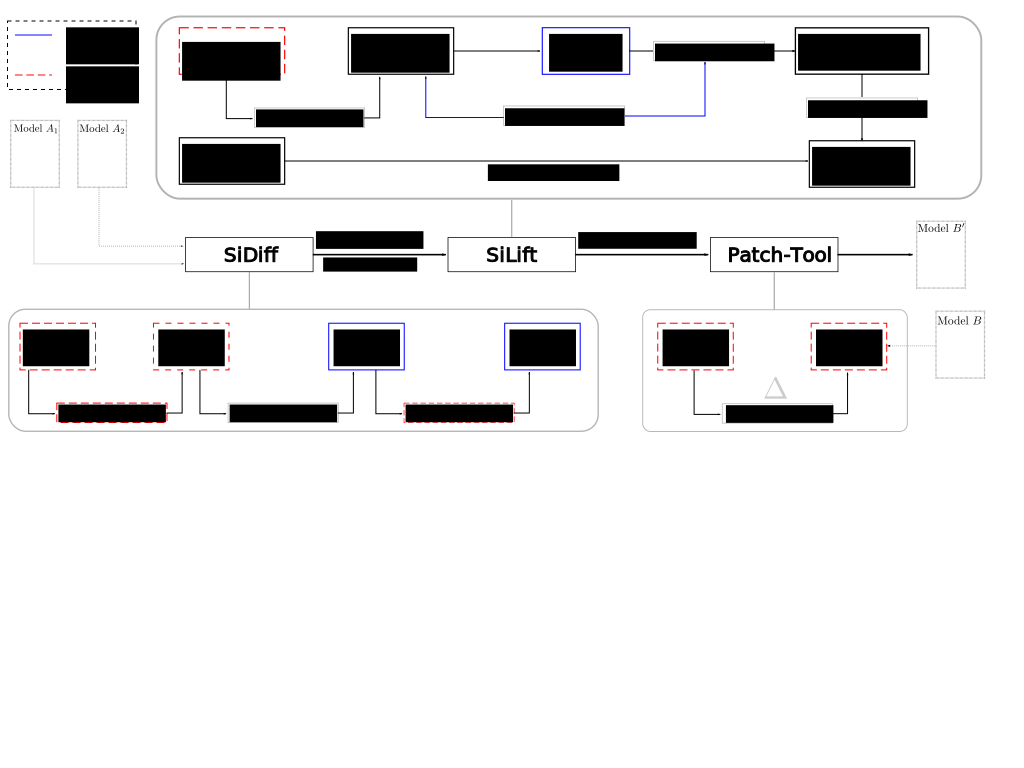
\includegraphics[scale=0.5, angle=0]{integration_overview}\\
\end{center}
\caption{UML profile integration overview}
\label{integration_overview}
\end{figure}
The tool pipeline can be described coarsely via the following steps:
\begin{enumerate}
  \item Two models $A_1$ and $A_2$ are given as input models.
  \item SiDiff creates a symmetric difference between them.
  \item SiLift lifts the low-level changes to more meaningful edit operations.
  \item The Patch-Tool deduces a patch and applies it to a target model $B$.
  \item The final result is a patched model $B'$ containing the changes
  detected between model $A_1$ and $A_2$ in model $B$ .
\end{enumerate}
As demonstrated in figure~\ref{integration_overview}, every tool has been
adapted for supporting \ac{UML} profiles, whether it be just modifications on
existing tools and services or creation of new ones. The concepts of this
adaptions will be presented in the following sections.
\section{SiDiff Integration}\label{Integration:sidiff}
The integration of \ac{UML} profiles into SiDiff and adaptions in general
can be divided into the following parts:

\textbf{\ac{UUID} Matcher}\\
The SiDiff matching pipeline has been adapted for better matching results if
elements of the input models contain \ac{UUID}s. Instead of just using one of
the matching services described in section~\ref{environment_and_tools:sidiff}, the
\ac{UUID} matching service is executed before the similarity-based matching
service. Therefore additional correspondences are already existent for the
following matching part, as shown in figure~\ref{integration_overview} in the
SiDiff box with dashed lines on the left side. Because of additional
correspondences at the start of of the similarity-matcher, it can deduce better
matching results. The already computed correspondences are taken into
consideration and are used as \textit{fix points} for the remaining unmatched
elements. This adaption is not specific for \ac{UML} profiles, but has been
implemented in this Master's Thesis.

\textbf{Similarity Matcher}\\
For the later concepts of the \ac{UML} profile integration and better matching
results in general, the similarity-based matcher has been adapted via its
configuration files. The focus was the definition of SiDiff configurations especially for
\ac{UML} itself, which can be used in other contexts as well. A snippet of such
a configuration is depicted in listing~\ref{sidiffcfg_example}.

\lstset{
    language=XML,    
    morekeywords={name,class,threshold,weight,parameter},
    caption={Snippet of \ac{UML} SiDiff configuration},
    label=sidiffcfg_example
    }
\lstinputlisting[firstline=633,lastline=640]{attachments/org.sidiff.sysml.core.compareconfig.xml}
In this example the matcher is configured for an \ac{UML} \textit{Class}
element, which will be matched after its attribute \textit{name}(l2-l3) and its
relationship to its \textit{parent} and \textit{children}(l4-l8). By adjusting
the weight between the configured elements, the results of the matching may improve or get worse.
This is just a small example of the vary configuration possibilities SiDiff has to offer. For a more detailed look into the possible SiDiff configuration parameters concerning the similarity
matching service contacting the \ac{SEG} via \cite{SEGURL} is suggested. As the
adaption of the \ac{UUID} Matcher, the improvement of the similarity-based matching
configuration for \ac{UML} is independent from the integration itself.

\textbf{Profile Matcher}\\
Profiled elements, conforming to the additive manner of \ac{UML} profiles, are
constructed as shown in figure~\ref{profilematcher_example1}: The base element
taken from \ac{UML}, in this case \textit{Class}, is extended by a newly defined
element, \textit{Block} in this case. Their relationship is defined via the
\textit{base\_Class} reference, which is a particular reference name used by
\ac{UML} profiles.

\begin{figure}[h!]
\begin{center}
\includegraphics[scale=1.0]{profilematcher_example1}\\
\end{center}
\caption{Example of two profiled models}
\label{profilematcher_example1}
\end{figure}

To describe the concept behind the developed profile matcher, two scenarios
concerning the example including model $A$ and model $B$ in figure~\ref{profilematcher_example1} can be imagined:
\begin{itemize}
  \item[a)] All elements contain \ac{UUID}s and they are corresponding to each other.
  \item[b)] One or all elements own a different \ac{UUID} or none at all.
\end{itemize}
In case a), which is presented in figure~\ref{profilematcher_example1}, the
newly integrated \ac{UUID} matcher will match corresponding elements. The
following execution of the similarity-based matcher will not add any new
results as already all possible correspondences have been found in the earlier
matching phase. Considering case b), in the similarity-based matching phase
there are unmatched elements because of wrong or missing \ac{UUID}s. Newly
introduced elements like \textit{Block} might be unmatched, in which case SiDiff
needs a feature to match those elements. To match profiling elements, there are
two possible solutions at hand:
\begin{enumerate}
  \item \textbf{Making use of the similarity matcher}\\  
  		Whereas at first sight this options seems more appropriate, the usage of the
  		similarity-based matching service depends highly on its configuration. As
  		explained beforehand, this configuration defines weighted elements and
  		attributes which should be taken into consideration for matching results. If
  		one element does not have much of its own semantics which can be considered
  		as important properties, the similarity matcher can not deduce meaningful
  		matches, which leads to wrong or missing correspondences between two models.
  		Taking figure~\ref{profilematcher_example1} into consideration, a element of
  		the type \textit{Block} does only define one boolean as own additional
  		attribute.
  		Comparing this attribute of model $A$, describing the additional semantics
  		of such \textit{Block}, to model $B$ one can clearly see that
  		this may lead to wrong correspondences. The only striking property of a \textit{Block} is the
  		reference to its base element. As such reference is always existent in
  		\ac{UML} profiling elements, the needed configuration of the similarity
  		matcher seems a unnecessarity. For each \ac{UML} profile and its elements
  		such a configuration part needs to be created, whereas they would contain
  		the same semantic content presented in listing~\ref{profiled_sidiffcfg}.
  		\lstset{
    language=XML,    
    morekeywords={name,class,threshold,weight,parameter},
    caption={SiDiff configuration for profiling elements},
    label=profiled_sidiffcfg
    }
    \begin{lstlisting}
    <Class name="Block" threshold="1.0">		
		<CompareFunction class="Parent" parameter="ECMatchedOrSimilar" weight="1.0"/>
		</Class>\end{lstlisting}
  \item \textbf{Implementing a new matching service}\\
  		Instead of using an available matching service, an additional matcher can be
  		introduced for supporting \ac{UML} profiles. As presented in
  		figure~\ref{integration_overview} an additional matcher for \ac{UML}
  		profiles has been developed and will be executed after the other matching
  		services provided by SiDiff. The basic idea behind the profile matcher is to
  		use all correspondences already created by other matchers and deduce results
  		concerning profiling elements from the former.
\begin{figure}[h!]
\begin{center}
\includegraphics[scale=1.0]{profilematcher_example5}\\
\end{center}
\caption{Concept of implemented profile matcher}
\label{profilematcher_example5}
\end{figure}

		The concept of the introduced profile matcher is shown in
		figure~\ref{profilematcher_example5}: The red marked boxes and correspondences
		have been created through the matchers prior in the SiDiff pipeline like the
		\ac{UUID} matcher or similarity matcher. If two elements are corresponding, which serve as base
		elements for profiling elements like in this case, the profiling elements
		marked in blue are also considered as corresponding. In this case the
		\ac{UML} configuration for SiDiff is crucial for good matching result, as
		the semantics of the base elements is used through the similarity matcher for
		matching the profiling elements. The profile matcher itself needs only a very minimal configuration
		effort, instead of the first variant using the similarity-based matching
		service. A detailed explanation of how this service is implemented and
		configurated can be found in section~\ref{realization:profilematcher}.
\end{enumerate}
\textbf{\ac{UUID} Fixer}\\
As the first two adaptions described in this chapter, this additional service
can be separated from the integration of \ac{UML} profiles. The \ac{UUID} fixer
service, as the name suggests, has been created for fixing wrong \ac{UUID}s
between corresponding elements. An explanatory example for a use case of the new
implemented service is presented in figure~\ref{wrongUUIDs_examples_p3}: Two
corresponding \textit{Associations}, namely Association2 and Association3, own
different identifiers. This can happen if an element has been deleted by the
developer and afterwards created newly again, representing the same semantics.
Many modeling tools rely on \ac{UUID}s and their correctness, whereas the
similarity matcher of SiDiff does not and creates such a correspondence
correctly. The new \ac{UUID} fixing service now corrects all \ac{UUID}s which
are mismatching, in this case it would replace the identifier of
Association3 with the one of Association2. Whether to change the \ac{UUID}s the
other way round is arguable, but the premise is to have two
consecutive revisions of software. In such a particular case, the identifiers in
the newer revision should be fixed instead of the ones in the older revision,
which would ruin all comparison possibilities with even older revisions.

\begin{figure}[h!]
\begin{center}
\includegraphics[scale=0.4]{wrongUUIDs_examples_p3}\\
\end{center}
\caption{Wrong \ac{UUID} example}
\label{wrongUUIDs_examples_p3}
\end{figure}

The service itself can be executed at any time considering the matching
pipeline, whereas its results are the best possible if executed at last.
By using this new service SiDiff itself offers a new feature, which has been
absent beforehand: Instead of supporting only matching of elements, SiDiff now
can fix wrong models and therefore make them yet again compatible to other
tools, which depend heavily on correct \ac{UUID}s.

For using all adapted and newly created tools together described in this section,
one can image following steps referring to the example in
figure~\ref{profilematcher_example1}, whereas the identifiers of the
\textit{Block} elements should differ:
\begin{enumerate}
  \item Both classes are matched by the \ac{UUID} matching service as they own
  the same identifier.
  \item The similarity-based matching service will not find any additional
  correspondences, because blocks are not part of the \ac{UML} configuration for
  SiDiff.
  \item Using the profile matcher, both blocks are matched because their
  respective base element \textit{Class} has been matched beforehand.
  \item Finally, the \ac{UUID} fixing service is executed and will replace the
  identifier of the \textit{Block} in model $B$ with the one of model $A$.
\end{enumerate}
Afterwards a generic \ac{UUID} matcher is capable of matching all elements,
including profiling ones like \textit{Block} in this example.
\section{SiLift Integration}\label{Integration:silift}
The integration of \ac{UML} profiles into SiLift translates to an integration
of \ac{UML} profiles into Henshin edit rules. If these rules are providing
support for profiled elements, then SiLift provides this support as well.
As already seen in figure~\ref{profilematcher_example1}, do profiled elements
essentially consist of themselves besides the relationship to their respective
base element. These two components need to be integrated into Henshin edit
rules, which can then be used by SiLift for its purposes. To achieve this goal,
three different variants can be deduced which are presented in
figure~\ref{variants_overview} using \ac{SysML} as applied \ac{UML} profile.

\begin{figure}[h!]
\begin{center}
\includegraphics[scale=1.0]{variants_overview}\\
\end{center}
\caption{Overview of different integration variants}
\label{variants_overview}
\end{figure}

\begin{enumerate}
  \item[Variant 1] \textbf{Integration into \ac{SERGe}}\\
 \ac{SERGe} is already capable of generating atomic edit rules by analyzing the
 corresponding meta model, including all \textit{set}, \textit{create}
 and \textit{delete} edit operations possibly executable by developers. Although
 \ac{UML} itself is supported by \ac{SERGe}, the profiling mechanism is not. The
 generator has to be adapted, to generate atomic edit rules, which contain the
 base elements as well as the profiling elements. The crucial advantage of this
 variant is the automated process of generating edit rules, whereas on the other
 hand new manually created edit rules can not be covered by this variant.
 Because of this drawback this variant has not been implemented in this Master's
 Thesis.
  \item[Variant 2] \textbf{Merging of Henshin rules}\\
  Another feasible solution is the merging of Henshin rules. The concept behind
  this idea is to take two rules, one containing only the base element and its
  properties, the other containing only the profiling element, and merge them
  into one resulting rule. Whether both rules have been generated or manually
  created does not concern, the drawback of the first variant is therefore absent.
  One difficulty to overcome in this variant is the merging of the rules
  itself: Finding the corresponding intersections between two rules as
  well as mapping parameters between them is complex in detail. Implementing
  this variant generically which does not only support the merging of Henshin
  rules for \ac{UML} profiles but rather supports the merging functionality for
  such Henshin rules in general makes this variant substantial sophisticated.
  Another mentionable disadvantage is the manual intervention for merging rules:
  The tool user has to be an expert on the used modeling domain, as he must
  define which rules should be merged into each other. These disadvantage have
  led to the following variant as solution, whereas this 
  variant could be taken into consideration for future work as presented in
  chapter~\ref{conclusionfuturework}.
  \item[Variant 3] \textbf{Adding profiling elements to existing Henshin rules}\\
  This variant has been implemented as part of this Master's Thesis as a service
  called \textit{ProfileApplicator}. Instead of merging two edit rules into one 
  as presented in variant 2, one pure edit base edit rule is taken as input and 
  transformed into a profiled one, containing profiling elements. This variant
  offers the same advantage like variant 2, the possibility of profiling
  manually created edit rules that is. Another advantage is the reduced complexity of
  development compared to the previous variant. Contrary to the merging variant,
  in this variant no manual intervention is needed in the creation process of
  the profiled rules, only a minimal configuration is needed for the
  ProfileApplicator to work instead. The concept of this variant is described in
  detail in the following section.
\end{enumerate}
\textbf{ProfileApplicator}\\
Adding profiling elements to a given model, which can be a Henshin rule itself,
can be achieved via a transformation. As Henshin is used in SiLift extensively
it has been chosen as the tool of choice for transformating such models. A Henshin
rule itself is a model, and therefore can be transformed like any other input
model. Such transformation is called \ac{HOT}, as it uses Henshin rules to
transform Henshin rules. An introductory result example of the execution of such
an \ac{HOT} is depicted in figure~\ref{hot_example}: The given edit rule on top
contains only the base element \textit{Class}, whereas the execution of a
\ac{HOT} adds the profiled element \textit{Block} to it resulting in the edit
rule shown below. 

\begin{figure}[h!]
\begin{center}
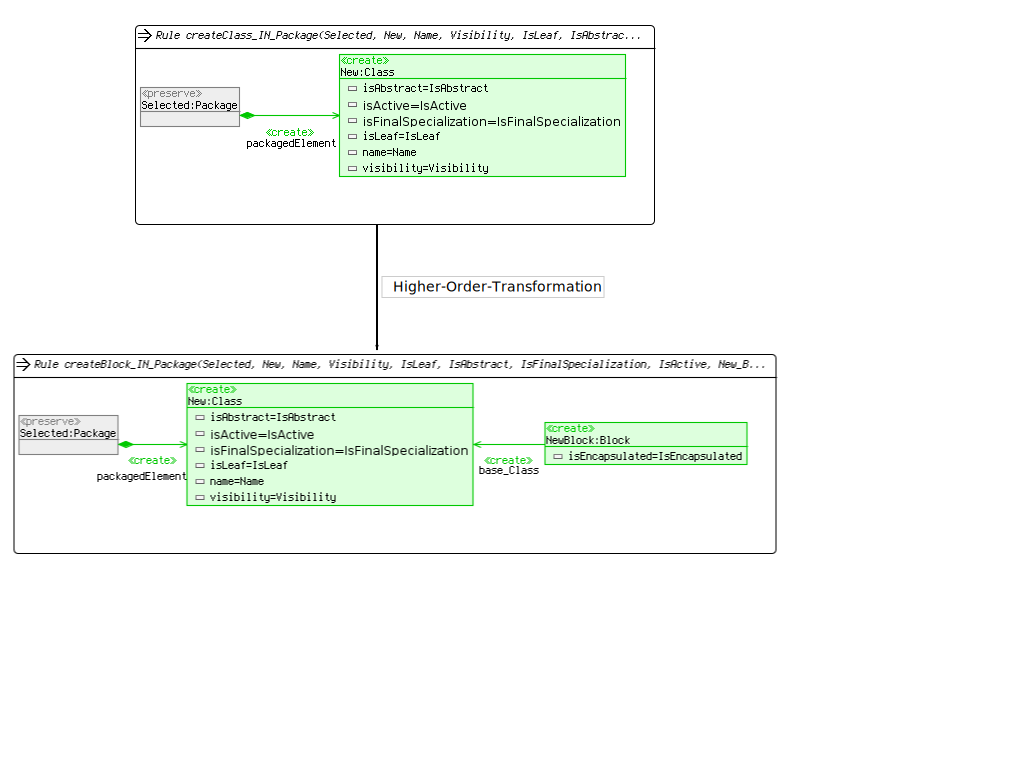
\includegraphics[scale=0.5]{hot_example}\\
\end{center}
\caption{\ac{HOT} example result}
\label{hot_example}
\end{figure}

This concept is implemented in the tool \textit{ProfileApplicator},
which executes such \ac{HOT}s for transforming given edit rules, such as
\ac{UML} edit rules.
As explained in section~\ref{environment_and_tools:henshin}, do Henshin rules
consist of three types of nodes: Create, delete and preserve. For each node type
a \ac{HOT} has been implemented, they can be found in
appendix~\ref{appendix:hots}. One exemplary rule covering the create nodes
depicted in figure~\ref{hot_create} will be explained in the following
paragraph.

Assuming the input model is an instance of a Henshin rule, the \ac{HOT} matches
a Module, which consists of one \textit{Unit} and one \textit{Rule}. Parts
of name and description attributes are replaced by a given String, this is just
a convenient renaming to identify profiled result rules more easily.
Additionally will the \ac{HOT} match a create node contained in the
\ac{RHS} graph and equals to the defined \textit{base type}, which is deducted
from the meta model of the \ac{UML} profile. If successful the following
elements will be created by this \ac{HOT}:
\newpage
\begin{itemize}
  \item A Create node of type \textit{stereo type} which has been derived from
  the meta model.
  \item An edge between the newly created node and the matched node of type
  \textit{base type}.
  \item All attributes of the stereo type node, except the ones defined as
  \textit{unchangeable}, \textit{derived} or \textit{transient} using a nested
  rule.
  \item New parameters in both the Henshin rule and unit.
  \item A parameter mapping between these two parameters.
\end{itemize}
The forbid node and edges are required for multiple executions of this \ac{HOT},
as there shall only be one profiled element of the same type be added to the
base element at most. If this \ac{HOT} is applied to the edit rule shown in the top of
figure~\ref{hot_example}, the rule below will be the result.

The remaining two \ac{HOT}s are defined in an similar manner, whereas some
differences can occur. The transformation of preserve nodes has to take also
the \ac{LHS} graph into consideration for example. Which base types will be used
as parameter can be configured in detail as will be seen in
section~\ref{realization:profileapplicator}.

 \textbf{Manually created edit rules}\\
 Although \ac{SERGe} does generate atomic edit rules by analyzing the
 corresponding meta model, not all rules containing the semantics are resulting.
 One example can be given in the area of the \ac{UML} concerning its
 representation of associations. An association is represented by two
 properties, which are either owned by the classes or by the association itself.
 Corresponding to optional relationships the meta model does not restrict the
 multiplicities, which results in \textit{wrong} generated edit rules. To cope
 with such special cases, one has to manually create such edit rules for
 themselves. One of the resulting rules is depicted in
 figure~\ref{atomic_example}: This edit rule is corresponding to the
 creation of an association which is navigable in one end. Such an association
 is defined via its properties, whereas one is owned by the corresponding class
 and the other is owned by the association itself. As part of this Master's
 Thesis different atomic manual rules have been created, which represent the
 semantics of the \ac{UML} meta model.
 
\begin{figure}[h!]
\begin{center}
\includegraphics[scale=0.55]{CREATE_Association_Navigable_ONE}\\
\end{center}
\caption{Manual atomic edit rule example}
\label{atomic_example}
\end{figure}

 Additionally to atomic edit rules, a domain expert can create complex edit
 rules, which have been defined in section~\ref{environment_and_tools:silift}.
 Adding complex edit rules, containing atomic edit rules, results in a better
 lifting possibility, which aids the developer at understanding the model more
 easily, as less edit operations are presented. One of the created rules is
 depicted in figure~\ref{complex_example}. As a special feature, this complex
 edit rule is modeled in \ac{SysML} instead of being modeled in \ac{UML} and
 transformated using the \textit{ProfileApplicator}. The reason for this is the
 added attribute \textit{direction} of the profiling element \textit{FlowPort}.
 This allows to define the direction of a given port and is a brilliant example for adding new
 semantics to known elements. This complex edit rule covers the creation of an
 interacting \textit{Block}, which is connected via its flow ports. The semantic
 behind this kind of block is that it receives a type of element, processes it in any
 way and passes the block on to another element connected via the outgoing port.
 This type of block is often used in the \ac{SysML} domain, as it may contain
 mechanical elements corresponding to this semantics.
 
 \begin{figure}[h!]
\begin{center}
\includegraphics[scale=0.5]{CREATE_Block_Interacting_Via_FlowPorts}\\
\end{center}
\caption{Manual complex edit rule example}
\label{complex_example}
\end{figure}

After manually creating missing edit rules and transformating all \ac{UML}
atomic and complex edit rules into profiled ones the defined rule base for \ac{UML}
profiles is complete. Now every possible edit operation in a particular
\ac{UML} profile like \ac{SysML} can be lifted with SiLift.
\section{Patch-Tool Integration}\label{Integration:patchtool}
Now that the first two steps of the tool pipeline
(fig.~\ref{integration_overview}) has undergone the \ac{UML} profile
integration, the final step has to be taken into consideration, the adaption
of the Patch-Tool that is. The Patch-Tool is responsible for the following three
features, which have to be adapted:
\begin{enumerate}
  \item \textbf{Creation of a patch} \\
  		The creation of a patch depends on the completeness of the given rule base
  		consisting of edit rules as well as the dependency correctness between them.
  		The latter as well as the former has successfully been solved through the
  		manual creation of rules missing or describing wrong semantics.
    \item \textbf{Application of a patch} \\
    	The successful application of a patch can only be ensured, if all
    	operation parameters can be resolved and the order of operations is correct
    	concerning the dependencies among them. Whereas the latter has already been
    	solved through the last feature, the former can be ensured if the matching
    	is done via SiDiff, including the \ac{UML} configuration and
    	profile matcher. Using these services a matching between all corresponding
    	elements can be created and therefore the parameter bindings.
    \item \textbf{Correctness of the result} \\
    	The last feature is the validation of the correct application of the patch.
    	For this purpose the models $A_1$ and $A_2$ are used for the creation of
    	such patch. The patch is then applied to $A_1$ and the result $B'$ is
    	compared to $A_2$. If and only if $A_2 = B'$ the patch has been applied
    	correctly and the result model contains all changes included in the patch.
    	A graphical overview of this situation is presented in figure~\ref{patch_correctness}.
		\begin{figure}[h!]
		\begin{center}
		\includegraphics[scale=0.6]{patching_correctness}\\
		\end{center}
		\caption{Patch result correctness condition}
		\label{patch_correctness}
		\end{figure}
		
		Such correctness can be only be tested as final step by using model instances,
		like done in chapter~\ref{solution}.
\end{enumerate}
 
\ac{UML} profiles are now fully integrated in all pipeline
steps(fig.~\ref{integration_overview}) and can be used consecutively. 
This chapter shall describe the concepts only instead of presenting the results
using a real \ac{SysML} case study. The results are explained extensive in
\ref{solution}.



\chapter{Realization of Concepts}\label{realization}
Based on the concepts presented in the preceding chapter, this chapter
describes the implementation process of the newly created tools and services.
Problems and details specific for the implementation part such as complexity
analysis or architectural features are illustrated. The usage of these
implemented services and tools in the environment of the \ac{SEG} is
additionally focused.
\section{ProfileMatcher}\label{realization:profilematcher}
For supporting the matching of \ac{UML} profiles in SiDiff a new service
has been introduced as part of this Master's Thesis. As shown in
figure~\ref{profilematcher} the matcher itself is executed after all other
SiDiff matching services. The implementation itself is based on the Eclipse
plugin architecture, as the whole \ac{SEG} tool pipeline is evolved around this
ecosystem.

 \begin{figure}[h!]
\begin{center}
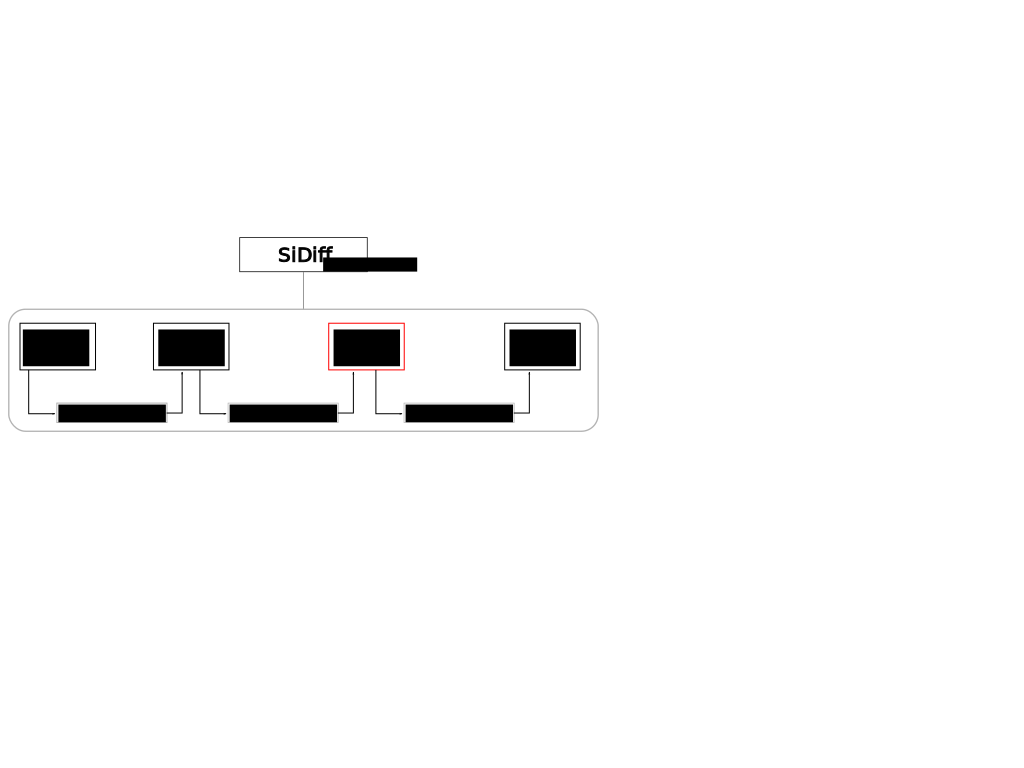
\includegraphics[scale=0.6]{profilematcher}\\
\end{center}
\caption{ProfileMatcher tool integration overview}
\label{profilematcher}
\end{figure}
\newpage

To integrate this service into tools using SiDiff, only a minimal change of code
has to be done by the tool engineer. Complying to the SiDiff service
architecture, the \textit{ProfileMatcher} can be integrated easily:
As described in section~\ref{Integration:sidiff} does the \textit{ProfileMatcher} rely on
computed correspondences, therefore the SiDiff \textit{CorrespondenceService} is
crucial for this matcher to work. Assuming this service has been registered
and is available for usage all needed lines of code to integrate and execute the
new matcher afterwards are depicted in listing~\ref{profilematcher_integration}.
 \lstset{ language=Java,
    caption={ProfileMatcher service integration},
    label=profilematcher_integration
    }
    \begin{lstlisting}
    //Define configuration file
    private final static String profileFileName = "uml.profiles.xml";
   
    //Configure ProfileMatcher according to configuration
    ServiceHelper.configureInstance(context, ProfilesMatchingService.class,
				UML_URI, null, profileFileName);
				
    //Register SiDiff service
  	ServiceContext.putService(ServiceHelper.getService(Activator.context,
  	ProfilesMatchingService.class, documentType, ServiceHelper.DEFAULT));
					
 	 //Execute ProfileMatcher service					
	 ServiceContext.getService(ProfilesMatchingService.class).match();\end{lstlisting}

As explained in detail in section~\ref{Integration:sidiff} one advantage of the
implemented matcher is the reduced effort needed for the configuration of
the service. The configuration syntax is based on other SiDiff
configurations like the one of the similarity matcher. The configuration of profiles is done like
depicted in listing~\ref{profilematcher_configuration}.

\lstset{
    language=XML,    
    morekeywords={name,encoding, base Package, stereo Package},
    caption={ProfileMatcher configuration example},
    label=profilematcher_configuration
    }
\lstinputlisting{attachments/org.sidiff.sysml.core.profileconfig.xml}

One configuration file can hold multiple \ac{UML} profiles such as the one
defined in line 4. Each profile can be configured in detail if necessary by
creating a white list of profiling elements, whereas the absence of such list
will use all existing profiling elements contained in the given \ac{UML}
profile, like done in listing~\ref{profilematcher_configuration}. The
matcher will iterate through all given profiles and match their white list
elements accordingly to their meta model automatically, therefore no additional
configuration is needed. The execution of the profile matching service will
engage the following actions for each configured profile:
\begin{itemize}
  \item Read the given configuration file and analyze the corresponding meta
  model according to this configuration.
  \item Save all profiling elements, their corresponding base element and the
  relationship reference between them in a map. 
  \item Build a map between both the profiling elements as well as the base
  elements.
  \item Iterate through all correspondences and search for base elements.
  \item Add a new correspondence to the respective profiling element if such
  base element is found in the correspondence as well as the built map.
\end{itemize}
\section{UUIDFixer}\label{realization:uuidfixer}
As the ProfileMatcher described in the preceding section, the \ac{UUID}Fixer is
implemented using the Eclipse plugin architecture and makes use of the SiDiff
service environment. 

 \begin{figure}[h!]
\begin{center}
\includegraphics[scale=0.6]{uuidfixer}\\
\end{center}
\caption{\ac{UUID}Fixer tool integration overview}
\label{uuidfixer}
\end{figure}

The integration part of this service is even more easily to be done, as there is
no need for any configuration at all(listing~\ref{uuidfixer_integration}). As
the ProfileMatcher, the \ac{UUID}Fixer makes use of the
\textit{CorrespondenceService} and is therefore most effective if executed as
last SiDiff service, as at this time more correspondences could be available.

 \lstset{ language=Java,
    caption={\ac{UUID}Fixer service integration},
    label=uuidfixer_integration
    }
    \begin{lstlisting}				
    //Register SiDiff service
  	ServiceContext.putService(ServiceHelper.getService(Activator.context,
  	IDFixerService.class, null, null));
					
 	 //Execute UUIDFixer service					
	 ServiceContext.getService(IDFixerService.class).fixIDs();\end{lstlisting}

The id fixing service algorithm can be divided into the following parts for each
model element $A$:
\begin{enumerate}
  \item Get corresponding element $B$ of current element $A$, if any.
  \item Compare the \ac{UUID}s of both elements $A$ and $B$ with each other.
  \item If they are not equal, replace the identifier of $B$ with the one of
  $A$.
\end{enumerate} 
As already denoted earlier, the replacement of the \ac{UUID} is done
in $B$ as it is the \textit{newer} model which is the one to fix. This
convention originates from the repository domain, as the fixing in $A$ would destroy
possible correspondences between $A$ and earlier revisions.
\section{ProfileApplicator}\label{realization:profileapplicator}
\begin{figure}[h!]
\begin{center}
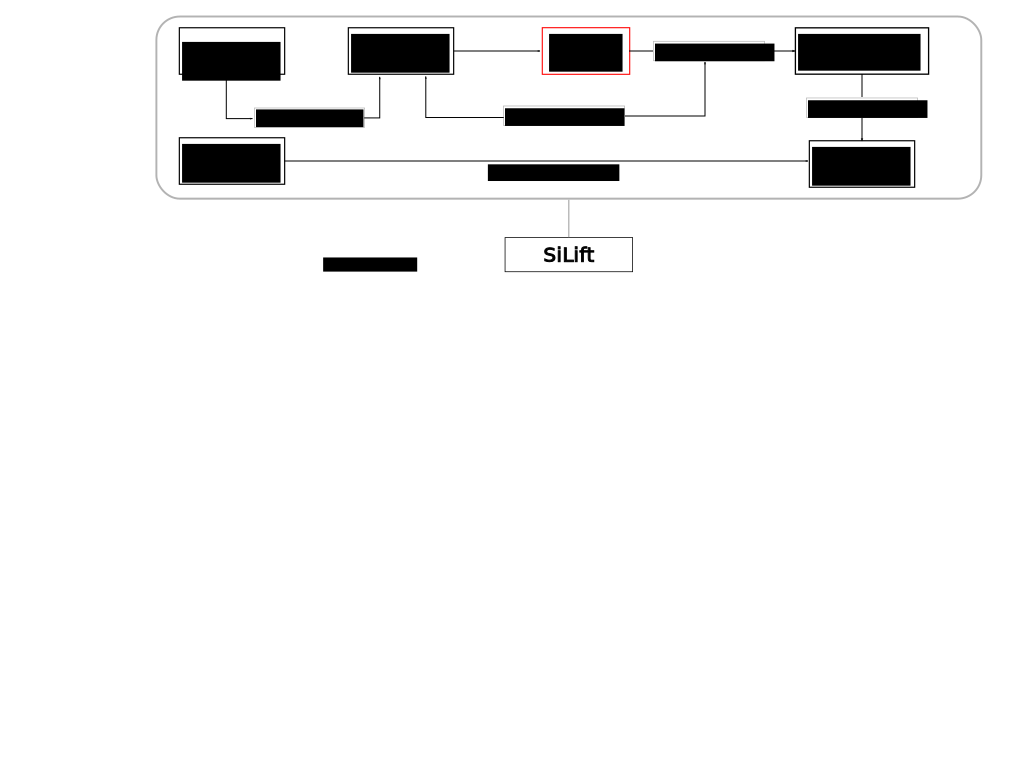
\includegraphics[scale=0.5]{profileapplicator}\\
\end{center}
\caption{ProfileApplicator tool integration overview}
\label{profileapplicator}
\end{figure}
Contrary to the previous services the \textit{ProfileApplicator} has been
implemented as an OSGi application, as it is used as standalone tool in the SiLift context.
The software architecture internally is similar to the one of \ac{SERGe}, as
they are used in the same manner and often even consecutively. As \ac{SERGe}
itself, the \textit{ProfileApplicator} has its own configuration for a detailed adaption
by the tool engineer, whereas the semantics of the configuration shall be
explained in detail. Considering the profile settings depicted in
listing~\ref{profileapplicator_profilesettings}, the following configuration
possibilities are available:

\begin{itemize}
  \item \textbf{Name} \\
  		This defines a human readable name for this \ac{UML} profile, which serves
  		as debug output and more understandable output possibilities in general.
  \item \textbf{BaseTypeInstances} \\
  		As the name suggests, does this option toggle the possibility of instances 
  		containing only the base element. As example the \textit{Class} /
  		\textit{Block} relationship seems appropriate: If the option is set to
  		\textit{false}, there shall be no \textit{Class} element without a profiling element \textit{Block}, whereas if set
  		to \textit{true} the result will be two edit rules, one containing only the
  		\textit{Class} element, the other containing both.
  \item \textbf{BaseTypeInheritance} \\
  		This option defines whether the ProfileApplicator should only take the
  		direct relationship and its corresponding base element of a give profiling
  		elements into consideration. Using \ac{SysML} as profile, the defined
  		element \textit{RequirementRelated} is added to every \textit{NamedElement}.
  		Disabling BaseTypeInheritance would result in no additional rule, as
  		\textit{NamedElement} is abstract and therefore cannot be instantiated. Enabling
  		would result in multiple result rules, as many concrete elements are of the
  		type \textit{NamedElement}, for example the \textit{Class} element.
\end{itemize}
\lstset{
    language=XML,    
    morekeywords={name,encoding,allow,nsUri,apply, basePackage, stereoPackage},
    caption={ProfileSettings configuration example},
    label=profileapplicator_profilesettings}
\lstinputlisting[firstline=4,lastline=8]{attachments/org.sidiff.profileapplicator.sysmlConfig.xml}
For additional adaption possibilities, the configuration part presented in
listing~\ref{profileapplicator_transformations} is available: The tool engineer
can decide which \ac{HOT} will be used by the \textit{ProfileApplicator},
declaring which type of Henshin nodes will taken into consideration for transformation.
\newpage
 \lstset{
    language=XML,    
    morekeywords={name,encoding,allow,nsUri,apply, basePackage, stereoPackage},
    caption={Transformations configuration example},
    label=profileapplicator_transformations}
\lstinputlisting[firstline=15,lastline=19]{attachments/org.sidiff.profileapplicator.sysmlConfig.xml}

Like the white list implemented in the profile matching service, does the
\textit{ProfileApplicator} also support this functionality. If none profiling element is defined, all
elements of the given \ac{UML} profile will be used. If on the other hand at
least one has been added, only these are used for transformation. This
configuration style has been used in \ac{SERGe} as well and therefore has been
implemented this way.

The execution of the tool needs additionally to the configuration
explained above two parameters, which can be defined by the user via an input
dialog presented by an OSGi execution configuration:
\begin{itemize}
  \item Folder of base type Henshin edit rules to transform (e.g. containing
  \ac{UML} edit rules).
  \item Target folder for saving the resulting transformed edit rules (e.g.
  \ac{SysML} folder).
\end{itemize}

While implementing the \textit{ProfileApplicator}, various runtime problems have
arisen, which needed a feasible solution. The transformation tool used by the
profile application tool is Henshin, which itself relies on Ecore~\cite{EcoreURL} for
internal model representation. Each \textit{EObject} loaded will register an
\textit{Action Listener}, which is capable of detecting changes concerning this
object.
Using the functionality on default, each \textit{EObject} will contain such listener and
each element referring to this EObject will create a
\textit{CrossReferenceAdapter}. Using large meta models like \ac{UML} will lead
to huge numbers of such adapters and listeners between all elements. This will
lead to an exponential growth while executing the ProfileApplicator, which
therefore will not finish its transformation in finite runtime. The solution is
presented as listing~\ref{listener_example}: All elements contained in an
\textit{EGraph} used by Henshin will be deleted manually, therefore all adapters
and cross references will be removed as well.
\newpage
 \lstset{ language=Java,
    caption={Deleting all EObjects manually},
    label=listener_example
    }
    \begin{lstlisting}
  public void releaseAdapters(EGraph graph) {		
    	for (EObject roots : graph.getRoots()) {
				graph.removeGraph(roots);
			}
	}\end{lstlisting}
	 
The deletion process uses some computation time itself, but the
the final runtime of the tool is constant and therefore ends
in finite runtime. Deleting these objects manually leads to the result shown in
figure~\ref{objectNumberReport} taken while executing the profile application.

 \begin{figure}[h!]
\begin{center}
\includegraphics[scale=0.5]{objectNumberReport}\\
\end{center}
\caption{Objects contained in an EGraph}
\label{objectNumberReport}
\end{figure}

Another runtime problem concerning the used \textit{EGraph} itself has arisen
during development. By default the constructor of such a Henshin EGraph will resolve
all object references of the given input model and will add the referenced
objects additionally to this EGraph. Given a large model like \ac{UML} as
input results in an enormous graph, which must be searched during the execution
of a Henshin rule. Henshin tries to match the preserve nodes as previously
described, whereas the number of nodes has a large impact on runtime. Adding
only the used elements into the EGraph manually instead of using the default
constructor leads to a considerable smaller EGraph and therefore runtime.
The code snippet of this solution is depicted in listing~\ref{egraph_solution}.
This solution reduced the EGraph size from $7463$ to $27$ for example, which
drastically effects the runtime.

 \lstset{ language=Java,
    caption={Manually adding needed elements to an EGraph},
    label=egraph_solution
    }
    \begin{lstlisting}
 	// Create Module EGraph and its children as working copy
	workGraph = new EGraphImpl();
	workGraph.addTree(workResourceSet.getModule(this.sourceFile.getName()));

	// Add all important elements for matching
	workGraph.add(applicator.getStereoPackage());

	// Add Stereotype and its Attributes
	workGraph.add(stereoType.getStereoTypeClass());
	for (EStructuralFeature feature : stereoType.getStereoTypeClass().getEAllStructuralFeatures()) {
		workGraph.add(feature);
	}
	
	//Add Basetype and baseReference
	workGraph.add(baseType);
	workGraph.add(stereoType.getBaseTypeMap().get(baseType));\end{lstlisting}

For further runtime improvement the ProfileApplicator implements the Java
threading technology as using threads in today's multicore environments seems
appropriate. Each profile applicator thread transforms one input Henshin edit
rule, therefore no concurrency problems can arise. Each input edit rule is
defined as work package which needs to be transformed. It is placed in a work pool, whereas each
thread can remove such a package for transformation. As the number of
threads used for computation are configurable via an execution parameter, 
each tool user can adapt this technology to his own needs. Having each thread
computed parallel reduces the runtime by a factor of threads e.g. having 4 threads 
executed on a quadcore processor leads to a runtime reduction by a factor close
to 4.

\chapter{SysML Case Study}\label{sysml}
The following chapter introduces a real world example of the \ac{UML} profile
\ac{SysML} in a detailed manner. At first an
introduction of the case study is given considering the semantics of the corresponding models.
Afterwards the case study is analyzed regarding technical and pragmatical issues
and their relevance related to modeling tools. This chapter lays the foundation
for chapter~\ref{solution}, in which the presented case study is used as exemplary input.
\section{Introduction}\label{sysml:introduction}
A real world case study concerning the domain of systems engineering presented by
the technical university of Munich in~\cite{aiscasestudy} has been modeled in
\ac{SysML}, as this \ac{UML} profile has been developed with such domain in
mind. The case study is evolved around a \ac{PPU}, which can be described as an
industrial automation plant. Its main purpose is the processing of given
elements like metallic pieces by picking them up and placing them onto a slide.
This scenario lays the foundation for the following revisions of this case
study and is depicted in figure~\ref{ppu_rev0}. The whole case study pursues
the target of demonstrating different iterations of a real world automation
\ac{PPU}, whereas the developers of this plant will add, remove or edit
elements throughout the revisions.

Revision 1, as shown in figure~\ref{ppu_rev1}, adds a new \textit{Y-Slide} to
the \ac{PPU} which will replace the simple slide of revision 0 and has to be
integrated into the semantics of the crane additionally for example. Now the
\ac{PPU} fills up both parts of this new slide as it increases the capacity for
work pieces. This is just a small example of the changes between each revision, a
more in-depth look at all revision changes can be taken in
the appendix~\ref{appendix:sysml_casestudy} or in the
publication~\cite{aiscasestudy}.

\begin{figure}[h!]
\begin{center}
\includegraphics[scale=0.4]{ppu_rev0}\\
\end{center}
\caption{\ac{PPU} case study revision 0~\cite{aiscasestudy}}
\label{ppu_rev0}
\end{figure}

The case study itself consists of 14 consecutive revisions each representing a
new version of the \ac{PPU} consisting of changes made by the developers.
The scope and the differences between each revision is
presented in figure~\ref{revisionChanges_analysis}: Revision 0 consists of
approximately 550 elements which are corresponding to revision 1
for example. As depicted via the blue graph, elements are mostly added which
finally leads to 1216 correspondences between revision 12 and 13. Noticeable
peaks of differences and therefore corresponding operations between revision 2
and 3 as well as 4 and 5 can be explained by the semantics of the changes: The
first peak corresponds to a new \textit{Stamp} module, which adds a
lot of new elements with its own semantics to the \ac{PPU} for example.

\begin{figure}[h!]
\begin{center}
\includegraphics[scale=0.6]{ppu_rev1}\\
\end{center}
\caption{\ac{PPU} case study revision 1~\cite{aiscasestudy}}
\label{ppu_rev1}
\end{figure}

Figure~\ref{revisionChanges_analysis} is the result of the combined usage of
all tools and services implemented as part of this Master's Thesis, whereas the results
themselves are presented in chapter~\ref{solution}.

\begin{figure}[h!]
\begin{center}
\includegraphics[scale=0.5]{revisionChanges_analysis}\\
\end{center}
\caption{\ac{PPU} revision changes overview}
\label{revisionChanges_analysis}
\end{figure}

\section{Analysis}\label{sysml:analysis}
Additionally to the semantics explained in the previous section, the \ac{SysML}
case study has been analyzed in detail regarding issues of different variants.
Several tools have been developed as part of this analysis, which shall not be
explained in this Master's Thesis as only their results are of importance. Three
types of issues have been defined, as they differ in impact on modeling tools and will be explained hereafter.

 \textbf{Technical Issues}\\
 Issues of this type have a crucial impact on modeling tools, as the results
 may differ distinguishably in absence of such issues. Whereas some modeling
 tools may deliver slighty wrong results, other modeling tools may deliver
 substantial wrong ones. Three examples of such issues found in the \ac{PPU}
 shall be given:
 \begin{itemize}
   \item \textbf{Wrong \ac{UUID}s}\\
   		 The example of
		 wrong \ac{UUID}s already given in figure~\ref{wrongUUIDs_examples_p3} shall
	 	 be recalled: The \ac{UUID}s of two corresponding associations in consecutive
	 	 revisions of the \ac{PPU} differ, as the association in the later revision
	 	 has been created newly by the developer. They describe the same semantics
	 	 thus both associations should be matched and the only change detected should
	 	 be a name change of the association. As many modeling tools rely on correct
	 	 identifiers, they would produce wrong results which differ extremely from
	 	 the expected. A summary of all wrong \ac{UUID}s found through all revisions
	 	 of this \ac{SysML} case study is shown in figure~\ref{wrongUUIDs_summary}.
	 	 The red bars are describing \textit{newly} created \ac{UUID} mismatches
	 	 between revisions, whereas the green bars present the number of wrong
	 	 identifiers carried over from older revisions.
	 	 	 	
		\begin{figure}[h!]
		\begin{center}
		\includegraphics[scale=0.6]{wrongUUIDs}\\
		\end{center}
		\caption{Summary of wrong \ac{UUID}s}
		\label{wrongUUIDs_summary}
		\end{figure}
		
  \item \textbf{Usage of EAnnotations}\\
  		\textit{EAnnotations} are available in Ecore models for annotating modeling
  		elements. They are defined like every other modeling element, therefore are
  		also considered during the detection of differences and correspondences
  		between models if absent. The case study is modeled in \ac{SysML} using
  		Papyrus\cite{PapyrusURL}, which will create EAnnotations for internal usage
  		of representation of associations as illustrated in
  		figure~\ref{eannotations}. Separating visual elements from semantic elements
  		is crucial in all areas of software development, especially in the case of
  		\ac{MDSD}. This is an example which problems can be caused if such
  		requirements are not met by modeling tools: Differencing between
  		two revisions which have been created with different tools will lead to
  		wrong results, as the EAnnotations added by Papyrus will cause differences.
  		\begin{figure}[h!]
		\begin{center}
		\includegraphics[scale=0.4]{eannotations}\\
		\end{center}
		\caption{EAnnotations created by Papyrus}
		\label{eannotations}
		\end{figure}
		
	\item \textbf{Usage of special characters}\\
		\ac{UML} does support the usage of special characters, which may
		cause problems in used modeling tools. Each modeling tool may handle these
		characters differently, as they may escape them with new ones or do not alter
		them at all. An example of the usage of such special characters can be
		depicted in listing~\ref{specialcharacter_example}: Papyrus itself escaped the
		character \glqq <\grqq\  by using the equivalent \glqq \&lt;\grqq\ whereas
		the opposite character \glqq >\grqq\ is not altered at all. These problems
		may cause problems at saving or loading the models, as the special characters
		are interpreted differently depending on the used modeling tool.
		
	\lstset{ language=XML,
    caption={Example of special character usage},
    morekeywords={xmi:type, xmi:id,name,encoding, basePackage, stereoPackage},
    label=specialcharacter_example
    }	
		    \begin{lstlisting}
 <subvertex xmi:type="uml:State" name="&lt;&lt;InCycle>>PickedUpState">
 	<doActivity xmi:type="uml:OpaqueBehavior" name="WPPickedUp:=TRUE;"> 
 		<language>Natural language</language>
 		<body>Kran_Sauger_an:=FALSE;&#xD; Kran_Sauger_aus:=true;</body>
  </doActivity>
 </subvertex>\end{lstlisting}
 \end{itemize}
 
\textbf{Pragmatical Issues}\\
This type of issues can be described as pragmatical, as they are not affecting
modeling tools and their result themselves but may lead to wrong understanding
of models by the developer. As described earlier, the \ac{SysML} case study has
been created using Papyrus, which makes use of its own diagram format. It
separates the view onto the models via its different diagrams from the
underlying model and offers the possibility to \textit{hide} modeling elements, which are
still present in the model itself. Unaware of consequences using this feature,
developers may hide elements in a particular revision, followed by another
developer not knowing of their existence in the model. This leads
to different pragmatical issues which have been categorized as follows:
	
\begin{itemize}
  \item \textbf{Missing elements}\\
  
\begin{figure}[h!]
\begin{center}
\includegraphics[scale=0.35]{missingElements}\\
\end{center}
\caption{Missing elements summary}
\label{missingElements}
\end{figure}
  		As mentioned before, hiding elements in a particular diagram view may lead
  		to the misunderstanding, that these elements do not exist within the model
  		itself. As shown in figure~\ref{missingElements}, there have been defined
  		two types of such elements:
  		\begin{itemize}
  		  \item[\underline{Undefined elements}] have to be defined in at least one
  		  diagram, for that the developer must know of their existence without the need of using
  		  other viewers as the diagram view itself. This category of elements has
  		  been further divided as depicted in figure~\ref{undefinedElementTypes}.
  		  Modeling elements described as undefined are important as they may change
  		  the understanding the model drastically. Examples of such elements are
  		  \textit{Block} or \textit{State}.
  		  
  		  \item[\underline{Global elements}] do not need to be defined in at least
  		  one diagram, as they are expected to be declared globally. This
  		  declaration can be imagined to be implemented outside of the given model,
  		  as these include elements such as \textit{Constraint} or \textit{Literal}.
  		\end{itemize}
	\begin{figure}[h!]
	\begin{center}
	\includegraphics[scale=0.35]{undefinedElementTypes}\\
	\end{center}
	\caption{Types of undefined elements}
	\label{undefinedElementTypes}
	\end{figure} 
	\newpage
  \item \textbf{Hidden model diagrams}\\
  		Hiding elements is not restricted to modeling elements as Papyrus provides
  		the feature of hiding particular diagrams at once. This leads to the same
  		problems described beforehand, whereas in this case more elements are
  		affected at one time. 
\end{itemize}



\section{Adaptions}\label{sysml:adaptions}
As described in the previous section, there have been found different
issues concerning the analyzed \ac{SysML} case study. Both technical and pragmatical
issues have been fixed in the course of this Master's Thesis for making all
revisions compliant to modeling tools and easing the understanding of these
models.
\begin{itemize}
   \item \textbf{Wrong \ac{UUID}s}\\
   		 Using the developed SiDiff services described in chapter~\ref{realization}
   		 all wrong \ac{UUID}s have been fixed and therefore no longer present a
   		 problem to modeling tools relying on identifiers.
   \item \textbf{Usage of EAnnotations}\\
    	 All used EAnnotations concerning tool specific information have been
    	 removed, as they may cause wrong results and do not provide any semantics.
   \item \textbf{Usage of special characters}\\
   		 Special characters, which may cause problems with modeling tools, have
   		 been stripped or replaced by semantically equal ones. The special
   		 character \glqq <\grqq\ has been replaced by the string \glqq
   		 LESSTHAN\grqq\ if this has been the desired semantics of this character
   		 for example.
   \item \textbf{Missing elements}\\
   		 All elements defined as global have been added to the Papyrus diagram
   		 view, so developers can understand the models themselves more easily.
   		 Global elements have not been added, as they may be defined elsewhere.
   \item \textbf{Hidden model diagrams}\\
   		 In the course of this Master's Thesis all hidden diagrams have been
   		 restored and can therefore be used and edited again.
\end{itemize}

After adapting the \ac{PPU} without altering the semantics of said models, the
case study presented in this chapter does not pose a problem to modeling tools
at all. The modified study has been used as exemplary input for all tools and
services created in the course of this Master's Thesis whereas the results are
presented in the following chapter.
\chapter{Solution Results}\label{solution}
This chapter illustrates the results of all implemented services and tools
created during this Master's Thesis by using a \ac{SysML} case study explained
in the preceding chapter. To achieve this all tools in the \ac{SEG}
pipeline are executed consecutively thus presenting the resulted integration of
\ac{UML} profiles using a real world example.

For testing the implemented solutions, one example scenario may be given
for this purpose.
Instead of using the \ac{PPU} scenarios 0 and 1 described in section~\ref{sysml:introduction}, the tools shall be tested with a more complex
revision change implemented in the \ac{SysML} case study.
Therefore both revision 2 and 3 are used, whereas the changes between them are
illustrated in figure~\ref{ppu_rev3}.

\begin{figure}[h!]
\begin{center}
\includegraphics[scale=0.4]{ppu_rev3}\\
\end{center}
\caption{\ac{PPU} case study revision 3~\cite{aiscasestudy}}
\label{ppu_rev3}
\end{figure}

The important difference between both model revisions is the addition of a new
\textit{Stamp} module. Only metallic work pieces should be stamped, whereas
black plastic work pieces are transported to the slide without being processed. To implement such
semantics, there has to be an additional sensor for detecting the position of
the stamp, whereas revision 2 already contains the inductive sensor for
differentiating between the two kinds of work pieces. The stamping process
itself is straightforward as one can imagine the movement of the stamp module
consisting of up and down alterations. Finally the crane transports the stamped
or unprocessed work piece onto the slide. A view illustrating the relationship
described beforehand can be seen in figure~\ref{ppu_rev3_uml}.

\begin{figure}[h!]
\begin{center}
\includegraphics[scale=0.6]{ppu_rev3_uml}\\
\end{center}
\caption{Revision 3 \ac{UML} diagram snippet}
\label{ppu_rev3_uml}
\end{figure}

As described in the Diploma Thesis of Dennis Koch~\cite{kochThesis}, one
practical aspect of the creation and application of patches is the propagation
of changes throughout different versions of software like a product family.
Considering this use case one can imagine two different automation plants $P_1$ and
$P_2$ each consisting of mentioned \ac{PPU} at revision 2. In need of such
functionality the customer owning $P_1$ wants the provider of the
\ac{PPU} to integrate the described stamp module. As $P_1$ now equals to
revision 3 depicted in figure~\ref{ppu_rev3}, the owner of $P_2$ wants to
have the same functionality for his plant. Instead of developing the exact same
model the developer wants to reuse his work done in $P_1$. To achieve this goal
all developed tools in this Master's Thesis are used consecutively, divided into
steps explained in the following paragraphs. For a better overview the tool
pipeline is yet again depicted in figure~\ref{integration_overview2}, whereas
the used model instance $A_1$ corresponds to $P_1$ and $A_2$ to $P_2$
respectively.

\begin{figure}[h!]
\begin{center}
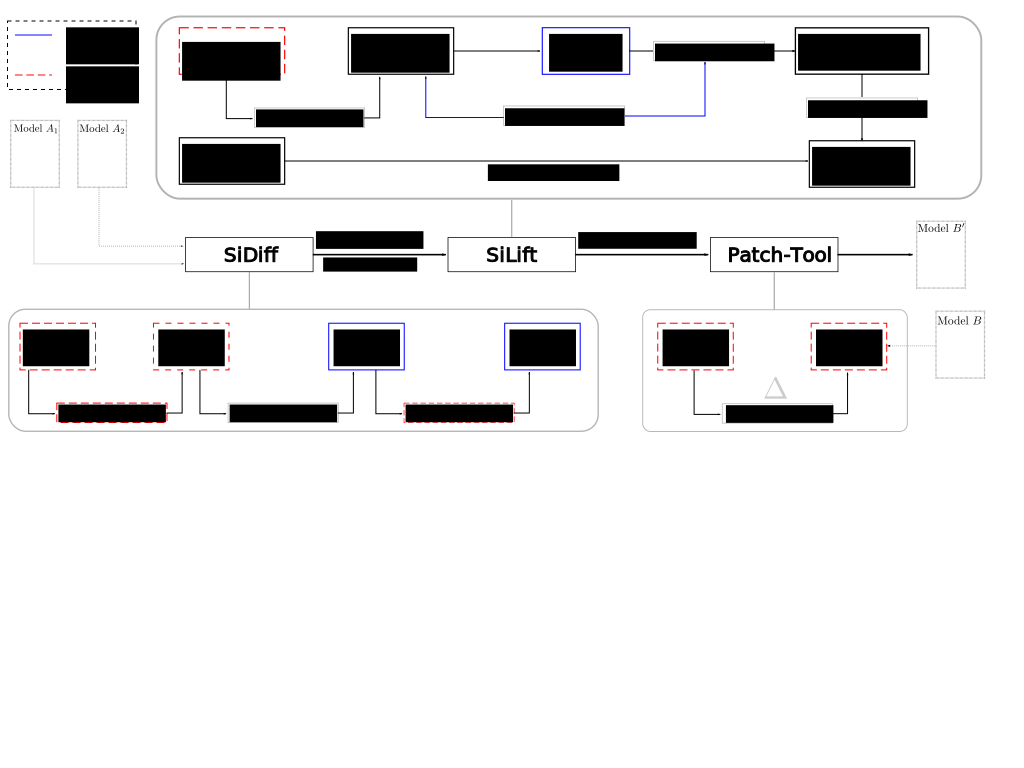
\includegraphics[scale=0.5, angle=0]{integration_overview}\\
\end{center}
\caption{UML profile integration overview}
\label{integration_overview2}
\end{figure}

\textbf{Compare $P_1$ and $P_2$} \\
The first step to the goal illustrated above is the detection of changes
between $P_1$ and the plant $P_2$. Using the SiDiff matching pipeline leads to
following results:
\begin{itemize}
  \item \textbf{\ac{UUID} Matcher}: 572 / 591 elements of $P_2$ matched, 785
  elements overall in $P_1$
  \item \textbf{Similarity Matcher}: 16 / 19 elements additionally matched
  \item \textbf{Profile Matcher}: 0 / 3 elements matched
  \item \textbf{Overall result}: 588 / 591 elements of $P_2$ matched, 197
  elements added in $P_1$
\end{itemize}

The first step matches all elements corresponding to their identifiers, whereas
in this example almost all elements could be matched already in this first
matching step. Using the \ac{UUID} matcher at first in this particular
case therefore leads to better results in the following similarity matching
phase. In this second matcher additionally 16 elements are matched according to their similarity. The final matching step for
profiled elements does not add any matches, as the remaining 3 elements are
originated from pure \ac{UML}. In the overall result for almost all elements of
$P_2$ have correspondences been found in $P_1$ which translates to only 3 delete
operations compared to $P_2$. Additionally 197 elements have been found in $P_2$
which correlates to newly added model elements in comparison to $P_1$. 
\newpage
\textbf{Analyze computed difference} \\
As the addition of a stamp block includes many other changes as well, the
developer now wants to analyze the detected differences and changes in detail.
First SiLift will derive low-level changes from the symmetric difference
computed by SiDiff. There are 764 low-level changes detected between $P_1$
and $P_2$ which need to be analyzed now if not lifted afterwards. To cope with
this many computed low-level changes the SiLift tool will lift this difference 
into a more meaningful list of edit operations. As seen in the center of
figure~\ref{integration_overview2}, SiLift now makes use of the profiled edit
rules created through the \textit{ProfileApplicator} as well as the manually
created edit rules. Using a complete rule base created earlier
for lifting will recognize edit operations like the manually created
depicted in figure~\ref{create_association_operation} and the profiled one in
figure~\ref{create_block_operation}.

\begin{figure}[h!]
\begin{center}
\includegraphics[scale=0.5]{create_association_operation}\\
\end{center}
\caption{Recognized manually created edit operation}
\label{create_association_operation}
\end{figure}

Low-level changes which are contained in such \ac{SCS}s will ease the
understanding of made changes as clearly presented in
figure~\ref{create_association_operation}: 14 low-level changes have been
grouped together into 1 meaningful edit operation, the creation of an
association which is navigable in one end that is.

\begin{figure}[h!]
\begin{center}
\includegraphics[scale=0.5]{create_block_operation}\\
\end{center}
\caption{Recognized profiled create operation}
\label{create_block_operation}
\end{figure}
\newpage
A result summary of all lifted low-level changes detected is
presented in the following table which reduces the number to 231 edit
operations instead of 758 low-level changes.\\
\begin{center}
{\footnotesize
\begin{tabular}{|l|r|}
Edit Operation & Amount\\
\hline
CREATE\_Transition\_IN\_Region\_(transition) & 49\\
CREATE\_State\_IN\_Region\_(subvertex) & 27\\
SET\_Transition\_(guard)\_TGT\_Constraint & 24\\
ADD\_Operation\_(method)\_TGT\_Behavior & 19\\
CREATE\_Constraint\_IN\_Transition\_(ownedRule)\_LiteralString\_ & 19\\
CREATE\_Activity\_IN\_State\_(doActivity) & 14\\
CREATE\_OpaqueBehavior\_IN\_State\_(doActivity) & 8\\
CREATE\_Pseudostate\_IN\_Region\_(subvertex) & 7\\
CREATE\_FinalState\_IN\_Region\_(subvertex) & 6\\
CREATE\_OpaqueBehavior\_IN\_State\_(entry) & 6\\
CREATE\_OpaqueBehavior\_IN\_Transition\_(effect) & 5\\
CREATE\_Association\_Navigable\_Property\_ONE\_Block(Class)\_IN\_Package & 5\\
UNSET\_Transition\_(guard)\_TGT\_Constraint & 4\\
CREATE\_Constraint\_IN\_Transition\_(ownedRule)\_LiteralBoolean\_ & 4\\
CREATE\_OpaqueBehavior\_IN\_State\_(exit) & 3\\
CREATE\_Operation\_IN\_Block(Class)\_(ownedOperation) & 3\\
SET\_Association\_Name & 3\\
SET\_State\_Name & 3\\
CREATE\_StateMachine\_IN\_Block(Class)\_(ownedBehavior) & 3\\
SET\_OpaqueBehavior\_Name & 2\\
SET\_Region\_Name & 2\\
DELETE\_Transition\_IN\_Region\_(transition) & 1\\
REMOVE\_Operation\_(method)\_TGT\_Behavior & 1\\
SET\_LiteralString\_Name & 1\\
DELETE\_Constraint\_IN\_Transition\_(ownedRule)\_LiteralString\_ & 1\\
MOVE\_Constraint\_(ownedRule)\_Transition & 1\\
SET\_Constraint\_Name & 1\\
CREATE\_Region\_IN\_State\_(region) & 1\\
MOVE\_State\_FROM\_Region\_(subvertex)\_TO\_Region\_(subvertex) & 1\\
SET\_Package\_Name & 1\\
CREATE\_Parameter\_IN\_Operation\_(ownedParameter) & 1\\
SET\_LiteralString\_Value & 1\\
SET\_Activity\_Name & 1\\
DELETE\_OpaqueBehavior\_IN\_State\_(doActivity) & 1\\
CREATE\_Block(Class)\_IN\_Package\_(packagedElement) & 1\\
\hline
 & \textbf{231} \\
\end{tabular}
}
\captionof{table}{SiLift lifting result summary}
\end{center}

\textbf{Create a patch} \\
Using the Patch-Tool the developer now wants to create a patch containing all
edit operations presented in the previous table. As the rule base is complete and all
low-level changes have been lifted by SiLift previously, all dependencies
between these are considered additionally. One example of such dependency
detected is illustrated in figure~\ref{dependency_example}: To create a
transition connecting two states both states have to be created first.

\begin{figure}[h!]
\begin{center}
\includegraphics[scale=0.5]{dependency_example}\\
\end{center}
\caption{Detected create-use dependency example}
\label{dependency_example}
\end{figure}

\textbf{Apply the created patch} \\
The next step is to apply the patch created beforehand to plant $P_2$, as this
plant shall implement the changes of $P_1$ compared to $P_2$. The application is
straightforward as presented in~\cite{kochThesis} and shall not be explained in
detail.

\textbf{Validate the resulted model} \\
The final step is to validate the resulted model. The developer wants to assure
that
\begin{itemize}
  \item[a)] the patch has applied all changes consistency preserving and that
  \item[b)] the resulted model equals to the expected result.
\end{itemize}

As the patch creation already assures a), the final step is to test the model
for its semantically correctness. To check for equality between $P_1$ and $P_2$
described in b) the SiDiff matching pipeline is used again and must report no
differences and all elements shall correspond as already presented in
figure~\ref{patch_correctness}.

\textbf{Final result} \\
The patch containing all changes could successfully be created and applied and
resulted in an equal plant implementing the stamp module, which is the desired
result. The patch can now be applied to different \ac{PPU}s for integrating such
new module.

Additionally to this example scenario between revision 2 and 3 of the \ac{PPU}
in the course of this Master's Thesis a batch application for testing all steps
above has been adapted for \ac{SysML}. The idea is to execute all steps for
consecutive revisions and log all results, which are shown in the
following table and correspond to the graphs in
figure~\ref{revisionChanges_analysis}.

\begin{center}
{\footnotesize
\begin{tabular}{|c|c|c|c|c|}
Revision Change & Correspondences & Differences & Operations & Equal\\
\hline
00$\rightarrow$01 & 545 & 58 & 16  & {\color{green}Yes} \\
01$\rightarrow$02 & 545 & 203 & 86  & {\color{green}Yes} \\
02$\rightarrow$03 & 575 & 764 & 231  & {\color{green}Yes} \\
03$\rightarrow$04 & 774 & 9 & 9  & {\color{green}Yes} \\
04$\rightarrow$05 & 756 & 654 & 201  & {\color{green}Yes} \\
05$\rightarrow$07 & 904 & 165 & 102  & {\color{green}Yes} \\
07$\rightarrow$08 & 927 & 103 & 28  & {\color{green}Yes} \\
08$\rightarrow$09 & 943 & 298 & 94  & {\color{green}Yes} \\
09$\rightarrow$10 & 1008 & 367 & 111  & {\color{green}Yes} \\
10$\rightarrow$11 & 1099 & 83 & 28  & {\color{green}Yes} \\
11$\rightarrow$12 & 1107 & 436 & 143  & {\color{green}Yes} \\
12$\rightarrow$13 & 1216 & 95 & 40  & {\color{green}Yes} \\
\hline
\end{tabular}
}
\captionof{table}{Batch-Patch summary report}
\end{center}

As illustrated in the table all revision changes can be handled now in all
tools in the \ac{SEG} pipeline, whereas all resulting patched models are equal
to their corresponding revision. The final conclusion of these results is
presented in the following chapter.
\chapter{Conclusion and Future Work}\label{conclusionfuturework}
This chapter concludes this Master's Thesis and offers an outlook for possible
future work based on the experiences gained throughout.

The integration of \ac{UML} profiles into the SiDiff and SiLift tools has
succesfully been achieved in this Master's Thesis. For the whole pipeline to
work with such profiled models all parts had to be adapted, namely:
\begin{itemize}
  \item Matching
  \item Lifting
  \item Patching
\end{itemize}
All three parts have successfully been adapted, whereas three new services and
tools have been introduced in this thesis:
\begin{itemize}
  \item \textbf{ProfileMatcher}\\
  		This services integrates \ac{UML} profiles into SiDiff and therefore allows
  		matching of such.
  \item \textbf{\ac{UUID}Fixer}\\
  		This new service allows for fixing of wrong identifiers and can be used for
  		compliance of models to other modeling tools.
  		\newpage
  \item \textbf{ProfileApplicator}\\
  		This new tool integrates \ac{UML} profiles into SiLift and therefore
  		lays the foundation for the lifting and patching functionalities.
\end{itemize}
After
the integration process in the course of this Master's Thesis the results have
been tested using a real world \ac{SysML} case study. First one example has
been introduced in detail and has been tested followed by a batch patch
application testing all revision of the whole case study. The final
result achieved is the successful  integration of \ac{UML} profiles as all tools
deliver the expected results, especially the final test for equality between
patched models and their corresponding revisions. The newly integrated support
for \ac{UML} profiles into SiDiff and SiLift increases their support of modeling
domains drastically, as many new modeling domains may arise by the aid of the
implemented profiling mechanism. Additionally the real world case study
created in \ac{SysML} can be used in future tools in this ecosystem, as it
represents a complex model and can be utilized for runtime tests for example.
The newly adapted \ac{UML} configuration for SiDiff can be used in other
contexts as well. A final overview of the results achieved in this Master's
Thesis are presented in figure~\ref{intergration_result_overview}.

 \begin{figure}[h!]
\begin{center}
\includegraphics[scale=0.5]{integration_overview_ready_p6}\\
\end{center}
\caption{Final integration result overview}
\label{intergration_result_overview}
\end{figure}
\newpage
The following aspects could be considered in future work:
\begin{itemize}
  \item \textbf{Testing of other profiles}\\
  		Additionally to the tested \ac{UML} profile \ac{SysML} others like
  		\ac{MARTE} can be used for testing, as their results may differ.
  		\ac{MARTE} makes use of own semantics in stereo types which needs to be adressed explicitly. One solution is the addition of
  		a new compare method for SiDiff which takes the similarity of stereo typed
  		elements into consideration.
  \item \textbf{Construction of edit rules}\\
 		To achieve better lifting result one can define more complex edit rules
 		than defined in this Master's Thesis for \ac{UML} itself or for a given
 		profile.
  \item \textbf{Implement remaining variants}\\
  		As in this Master's Thesis only variant 3 of the different integration
  		approaches into SiLift has been implemented, both remaining could be
  		implemented in the future. As depicted in figure~\ref{variants_overview} the
  		first variant would result in an integration into \ac{SERGe}, whereas the
  		second variant shall be implemented as own tool. Instead of supporting only
  		the merging of base and profiled edit rules one can implement such Henshin
  		rule merger generically and therefore support the merging of Henshin rules
  		in general. This would result in new possibilities like merging two atomic
  		edit rules into one complex rule without the need of manual intervention.
  \item \textbf{Performance optimizations}\\
  		As the newly supported \ac{SysML} case study can be described as complex,
  		some parts in the tooling pipeline shall be taken into consideration for
  		performance optimizations. This concerns elements like runtime or memory
  		consumption as well as user interface optimizations.
\end{itemize}

%------ appendix ------
\appendix
\chapter{Higher-Order-Transformations}\label{appendix:hots}
The following figures illustrate the in this Master's Thesis created \ac{HOT}s,
which transform given Henshin edit rules into profiled ones.
 \begin{figure}[h!]
\begin{center}
\includegraphics[scale=0.6, angle=90]{CREATE_STEREOTYPE_IN_EDITRULE}\\
\end{center}
\caption[]{\ac{HOT} for create nodes}
\label{hot_create}
\end{figure}
\newpage
\begin{figure}[h!]
\begin{center}
\includegraphics[scale=0.6, angle=270]{DELETE_STEREOTYPE_IN_EDITRULE}\\
\end{center}
\caption[]{\ac{HOT} for delete nodes}
\label{hot_delete}
\end{figure}
\newpage
\begin{figure}[h!]
\begin{center}
\includegraphics[scale=0.55, angle=90]{PRESERVE_STEREOTYPE_IN_EDITRULE}\\
\end{center}
\caption[]{\ac{HOT} for preserve nodes}
\label{hot_preserve}
\end{figure}
% \chapter{SiDiff UML configurations}\label{appendix:sidiffcfgs}
% \lstset{
%     language=XML,    
%     morekeywords={encoding, documentType,
%     normalizeWeights, condition, policy, name,class,threshold,weight,parameter},
%     captionpos=top, caption={SiDiff \ac{UML} similarity configuration},
%     label=sidiffcfg_similarity
%     }
% \lstinputlisting{attachments/org.sidiff.sysml.core.compareconfig.xml}
% \newpage
% \lstset{
%     language=XML,    
%     morekeywords={encoding, documentType,
%     normalizeWeights, condition, policy, name,class,threshold,weight,parameter},
%     captionpos=top, caption={SiDiff \ac{UML} matching Sequence},
%     label=sidiffcfg_similarity
%     }
% \lstinputlisting[firstline=99,lastline=130]{attachments/org.sidiff.sysml.core.matchingconfig.xml}
\chapter{\ac{SysML} Case Study Evolution}\label{appendix:sysml_casestudy}
This appendix describes the evolution of the \ac{SysML} case study used
throughout this Master's Thesis in a detailed manner. This evolution has been
created by the technical university of Munich and the corresponding
publication~\cite{aiscasestudy} is recommended.
\includepdf[pages={-}]{attachments/Description_EvolutionScenarios.pdf}

%***** Bibliographie  *****
%Die Literatur wird in einem eigenen Dokument im BibTeX Format erfasst: in diesem Fall: referenzen.bib
\bibliographystyle{plain}
\bibliography{bibliography}

\addcontentsline{toc}{chapter}{Bibliography}

%\include{literatur}


%------ end of document ------
\end{document}
